\documentclass[11pt, oneside]{article}   	% use "amsart" instead of "article" for AMSLaTeX format
\usepackage{geometry}                		% See geometry.pdf to learn the layout options. There are lots.
\geometry{a4paper}                   		% ... or a4paper or a5paper or ... 
%\geometry{landscape}                		% Activate for rotated page geometry
%\usepackage[parfill]{parskip}    		% Activate to begin paragraphs with an empty line rather than an indent
\usepackage{graphicx}				% Use pdf, png, jpg, or eps§ with pdflatex; use eps in DVI mode
								% TeX will automatically convert eps --> pdf in pdflatex		
\usepackage{amssymb}
\usepackage[dvipsnames]{xcolor}
\usepackage{hyperref}
\usepackage{float}
\usepackage{subcaption}

%SetFonts

%SetFonts


\title{Final Project - Meta Cognition}
\author{Gal Waisman and Sergiy Horef}
%\date{}							% Activate to display a given date or no date

\begin{document}
\maketitle
\begin{center}
	Code for the project - \href{https://github.com/Horef/mc_final}{GitHub}
\end{center}

\tableofcontents

\newpage
\section{Dataset}
Corresponds to points 1,2 in the requirements.
\subsection{Data Collection}
We have chosen to scrape Reddit for posts in the following subreddits:\\
r/: macapps, learnprogramming, learntodraw, learnpython, learnmath, LaTeX, Python, datascience, dataengineering, malefashionadvice, MachineLearning, ObsidianMD, neuroscience, printSF, science, ios, MacOS and mac.\\
We have chosen these subreddits, as we have noticed that they have a high amount of "question posts" (posts that have one or more correct answers).\\

We have scraped the data using python, and the following main libraries: 'selenium' and 'BeautifulSoup' (the code can be found in the github repository provided).\\
We have filtered the posts by their title, and only included the ones which have either "?", "question" or "help" in the title text.\\
Because reddit has a tree-like structure of comments - that is, each comment can have subcomments, etc. we have only included the comments which were made to the post itself, and therefore can be the possible answers.\\

For each comment we have collected the following information:\\
1. Score - difference between the likes and dislikes.\\
2. Replies - number of replies (sub-comments) for that comment.\\
3. Awards - number of awards (if any) that were given to the comment.\\
4. Length - number of symbols in the comment.\\
5. Length to Average Ratio - ratio between the length of a given comment to the average comment on that post. ($\frac{Length}{avg.Length}$)\\
We have not collected the text of the question or the answer itself, as this data would be much harder for the model to use, and would take much more time for the people to read.\\
Moreover, we have felt that the five numbers we have collected will be enough for the model to meaningfully train.\\


In total we have succeeded in collecting 1274 comments, out of which we have chosen 50 that would be used for model training and human labeling (level of sureness).\\
We have chosen these comments such that they would be "interesting" and include relatively high scores, length and reply numbers with the following statistics:\\
\begin{center}
	\begin{tabular}{|l|c|c|c|c|}
		\hline
		stat/value & score & replies & length & length ratio\\
		\hline
		min & -4 & 0 & 5 & 05.49\% \\
		mean & 93.74 & 2.36 & 118.74 & 64.78\% \\
		max & 1437 & 37 & 744 & 288.62\% \\
		std & 224.17 & 5.75 & 133.57 & 54.67\%\\
		\hline
	\end{tabular}
\end{center}

We have chosen not to include the "awards" value for each of the comments, as it has shown to be non-informative, with most values being a 0, and only a few being 1 or 2.\\

\subsection{Data Labeling}
In order to label the 50 coments we have chosen, we have split them into 2 groups of 25 each, and each was labeled by 5 different people.\\

Each person got a personal explanation of what the data represents, and how it was collected. Later, each one was shown an excel-like table, with each row representing an individual comment, and each column filled with the corresponding value of that measure ("score", "number of comments", "length", "length ratio").\\
Last column was empty, and represented the sureness (0-100\%) of the comment writer as estimated by the person. Each person was asked to fill this column based on their subjective feeling and understanding.\\

Later, each comment got its final label to be the average of 5 labels provided by the people in its group.
We have wanted to make the final labels an average of a few opinions, as otherwise intra-person bias could lead to an incoherent data.\\

The final labels follow the following statistics:
\begin{table}[H]
\begin{center}
    \begin{tabular}{|l|c|}
    \hline
    stat & value \\
    \hline
    min & 58.2 \\
    mean & 76.8 \\
    max & 92 \\
    std & 8.87 \\
    \hline
    \end{tabular}
\end{center}
\end{table}

Or in a box plot:
\begin{figure}[H]\label{fig:sureness_stats}
    \begin{center}
    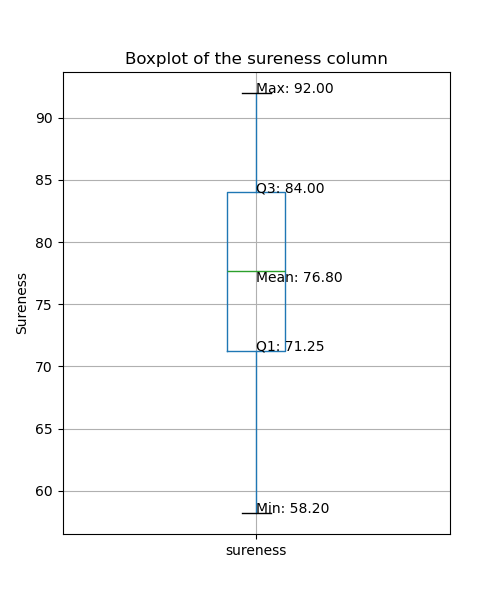
\includegraphics[height=0.7\linewidth]{../plots/sureness_boxplot}
    \caption{Statistics of the labeled data}
    \end{center}
\end{figure}


\section{Models and Results}
Training of all models can be found in 'main.py'\\
Corresponds to point 3 in the requirements.\\

We have not collected either the questions themselves, or the full text of the comments, therefore we could only use models that do not rely on natural human language.\\

\textbf{Models}: we have tried 5 different models: 1 baseline model, 3 simple ones of the "fit-predict" sort, and a simple neural network.\\ 
Each model was trained to predict a real number in range 0-100 to be as close to the "real" label (as explained in the previous section). In order to make sure that predicted values were valid, prediction of each model had an additional step which clipped all of the values to the 0-100 range.
We talk more about each model in the following subsections.

\textbf{Evaluation}: for each of the models we have done 5-fold cross validation, where the data was initially split into 5 (disjoint) sets of data points, with 10 points each. Later, each fold was used for testing, while other folds were unified and used for training of the model.\\
For each test, we have measured the mean l1 - mean absolute error (MAE), and mean l2 - mean squared error (MSE), between the predicted labels, and the "real" ones.

\textbf{Note}: in all models that have used any sort of randomness, and for the division into splits in cross-validation, we have used the seed of 3.

\subsection{Baseline}
Implementation can be found in 'Baseline.py'\\

From \hyperref[fig:sureness_stats]{labels distribution box plot} can be seen that even though the total range of the data is relatively big, ranging from 58 to 92 (92-58=34), most of the data is concentrated around the mean value of 76.8 (Q3-Q1=84-71.25=12.75 or one-sided: Q3-Mean=84-76.8=7.2).\\
Therefore, in order to check the real usefulness of other models, we have created a baseline model - when trained, it saves the mean value of the training labels, and on the test stage it simply always returns that value.\\

This model achieves \textbf{MSE of 79.27} and \textbf{MAE of 7.39}.

\subsection{K-Nearest Neighbors (KNN)}
Implementation can be found in 'KNearestNeighbors.py'\\

We have started by creating a weighted regression KNN model, implementation for which we have taken from the sklearn module. (Standard module for machine learning tasks.)
Given a point, this model finds $k$ nearest points in the training set, and returns a label which is the weighted (by l2 distance) average of the $k$ points.

We have tested all values of $k$ from 1 and up to 40 (always average all points), and found that the best result is achieved at $k=6$ with \textbf{MSE of 55.2} and \textbf{MAE of 5.89}.\\
That is, on average, this model returns labels that are 5.89 away (to either side) from the real value. Not bad!

Here is the plot of performance as a function of different values of $k$:
\begin{figure}[H]
\begin{center}
    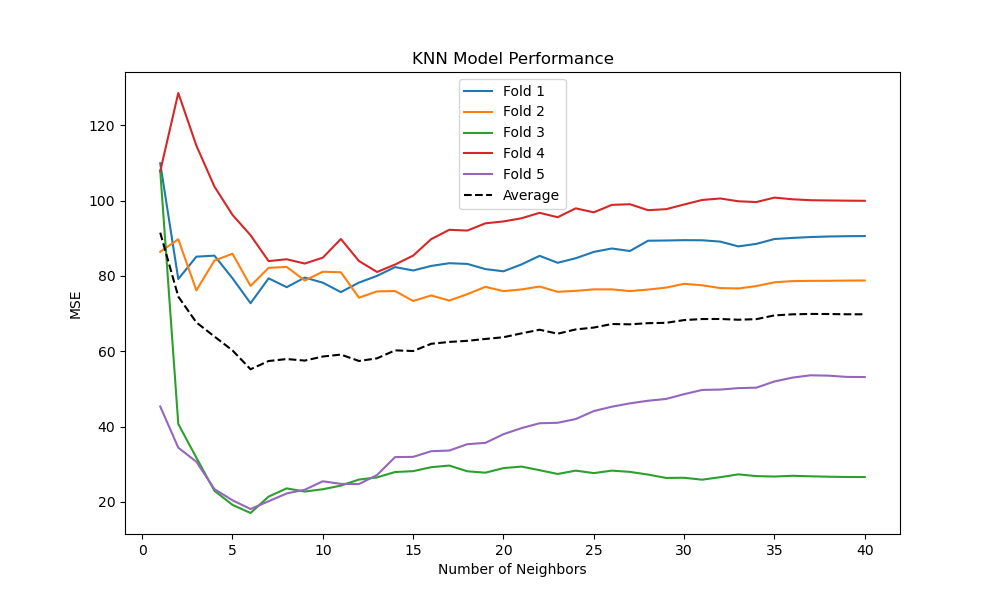
\includegraphics[width=0.65\textwidth]{../plots/knn_performance.png}
    \caption{Graph of KNN performance}
\end{center}
\end{figure}

\subsection{Decision Tree}
Implementation can be found in 'DecisionTree.py'\\

Next we have implemented a Regression Decision Tree (using sklearn).\\
Given a set of training points, this model creates a decision tree, where at each step it splits the data into two groups by value of one of the parameters. When a new point is classified, it moves through the tree until it reaches a leaf group, and receives a value which is the average of all values in that group.

We have tested all depths from $d=1$ and up to $d=20$, and found that the best result is achieved at $d=1$ with \textbf{MSE of 91.91} and \textbf{MAE of 7.74}. The tree for this depth looks like this:

\begin{figure}[H]
    \begin{center}
    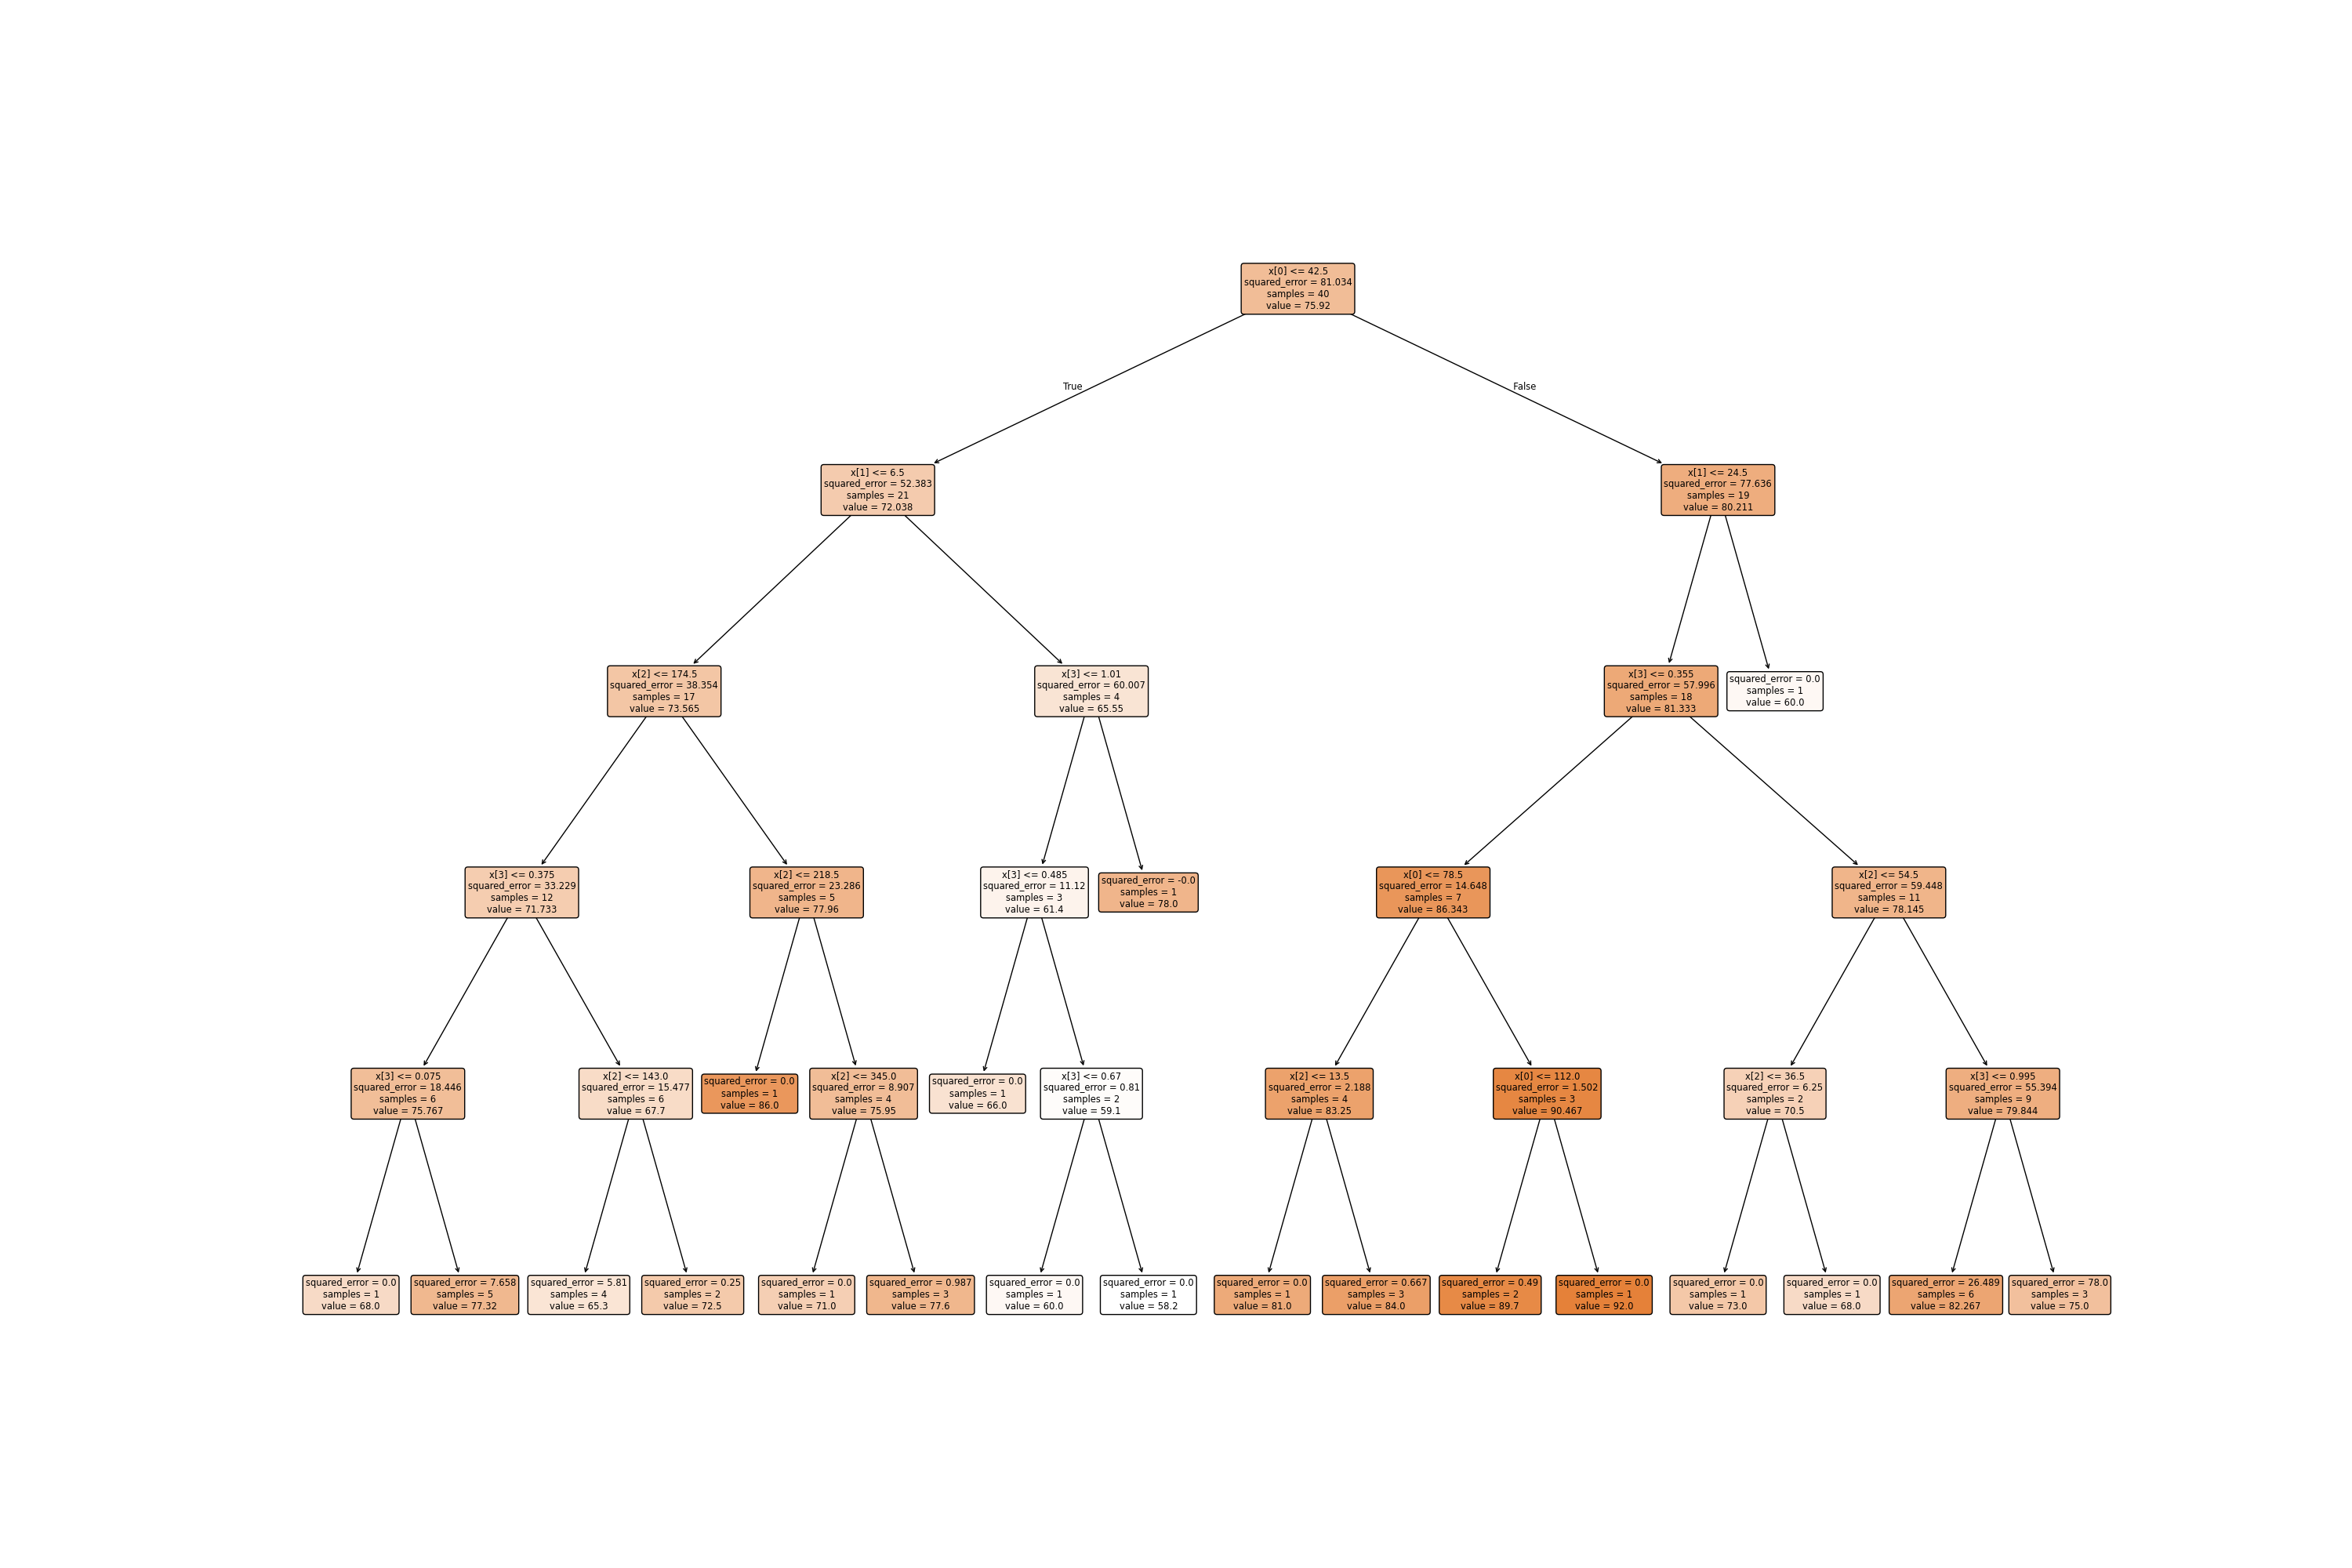
\includegraphics[width=0.55\textwidth]{../plots/decision_tree}
    \caption{Decision Tree of depth 1 (trained on folds 1-4)}
    \end{center}
\end{figure}
 
That is: the average over all labels is 75.92, and the split is done using the 'score' parameter. Anything that has a score of 42.5 or less, will be assigned a label of 72.038, and else a label of 80.211.

The overall performance of the Decision Tree model as a function of the depth:
\begin{figure}[H]
    \begin{center}
        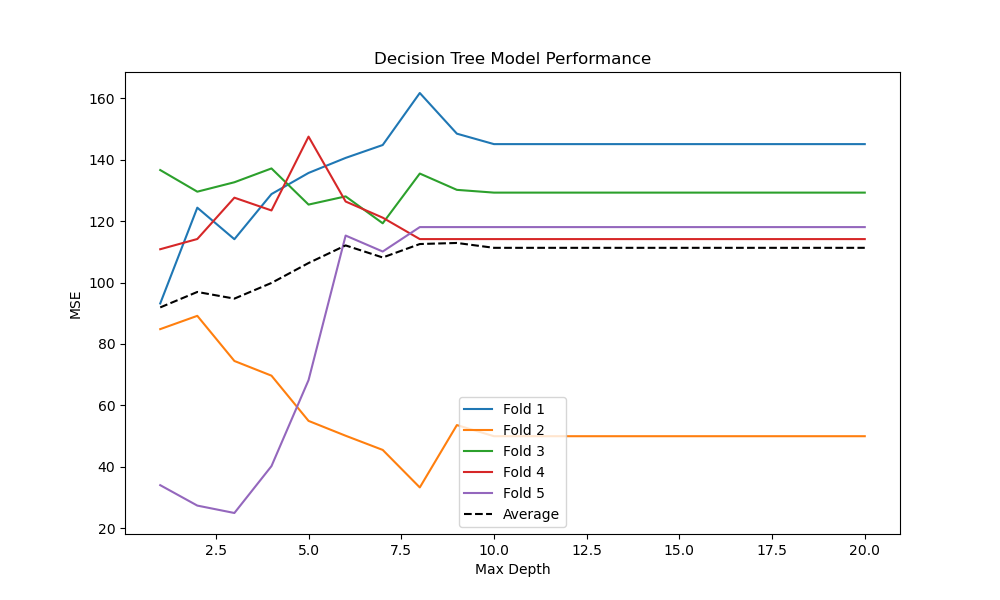
\includegraphics[width=0.65\linewidth]{../plots/decision_tree_performance}
        \caption{Performance of Decision Tree on various folds}
    \end{center}
\end{figure}

\subsection{Feed Forward Neural Network}\label{sec:ffn}
Implementation can be found in 'FeedForwardNetwork.py'\\

As we have only 40 points for each fold, training a deep learning model is impractical. As almost all of them are only relevant when the number of points is relatively high, or if the data is very homogeneous.\\
However we still wanted to see how a deep learning framework would perform, and therefore chose to train a simplest form of a feed forward neural network.

We have tested different numbers of layers from $n=1$ and up to $n=5$, and found that the best results were achieved over $n=3$ (size of the hidden layer is 9), with \textbf{MSE of 95.32} and \textbf{MAE of 8.11}. Much worse than the simpler models, but rather as expected.

Here is an example of the MSE and loss of the model on one of the folds:
\begin{figure}[H]
    \begin{center}
        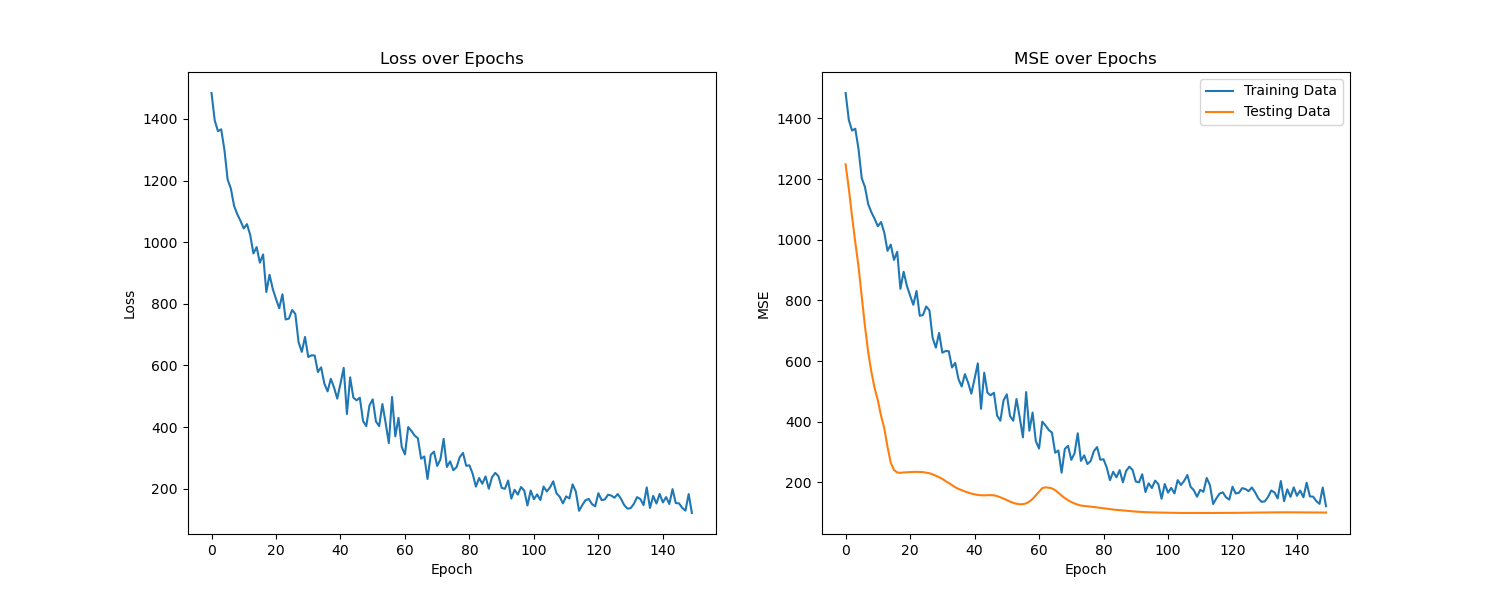
\includegraphics[width=\linewidth]{../plots/ffn_performance}
        \caption{Performance of an FFN on one of the folds}
    \end{center}
\end{figure}

We can clearly see that after around 90 epochs of training the model converges to its best result. (Even though this result is not really good.)

\subsection{Linear Regression}
We have used the LinaerRegression module implemented in sklearn.\\

As our last model, we wanted to train a Linear Regression model, to try and understand which factors (possibly) had the most effect on the label assigned by our friends.\\
Here are the results for each fold, with coefficient values, MSE and MAE:
\begin{table}[H]
\begin{center}
    \begin{tabular}{|l|c|c|c|c|c|c|}
    \hline
    fold/val & score & replies & length & length ratio & MSE & MAE \\
    \hline
    fold 1 & 0.0070 & -0.8193 & 0.0047 & -1.1185 & 82.62 & 7.62 \\
    fold 2 & 0.0073 & -0.4781 & 0.0086 & -2.0259 & 73.43 & 7.46 \\
    fold 3 & 0.0072 & -0.6053 & 0.0072 & -3.9961 & 50.07 & 6.67 \\
    fold 4 & 0.0078 & -0.4738 & 0.0038 & -1.3141 & 89.85 & 8.24 \\
    fold 5 & 0.1689 & -0.4822 & 0.0171 & -2.4431 & 107.49 & 8.52\\
    \hline
  \end{tabular}
  \caption{Coefficients and results of Linear Regression on different folds}
\end{center}
\end{table}
And on average, the results were \textbf{MSE of 80.69} and \textbf{MAE of 7.70}. This result is still much worse than what was achieved using the simple KNN, but is better than either Decision Tree or FFN.

\subsection{Intermediate Conclusions}\label{sec:inter_conclusions}
First of all, lets look at a general comparison between all of our models (the best values (less is better) are highlighted in bold):
\begin{table}[H]
  \begin{center}
  \begin{tabular}{|l|c|c|}
    \hline
    Model & MSE & MAE \\
    \hline
    Baseline & 79.27 & 7.39 \\
    KNN & \textbf{55.2} & \textbf{5.89} \\
    Decision Tree & 91.91 & 7.74 \\
    FNN & 95.32 & 8.11 \\
    Linear Regression & 80.69 & 7.70 \\
    \hline
  \end{tabular}
  \caption{Comparison of model performance}
  \end{center}
\end{table}

It can be clearly seen that only the KNN model can be said to have learned something, as all others perform worse than even the baseline, which does no computations whatsoever.\\
Linear Regression provides results that are close to Baseline, but are still a little worse.\\
Neural Network performs as expected given such a small training set - produces results that are much worse than any other model, and almost a whole unit farther than Baseline in the MAE value.\\

In light of all of the results, we can state a few conclusions:
\begin{itemize}
    \item The good performance of the KNN model suggests that the heuristics our friends have used in order to label each example were conditional on a few similar, or previously labeled, examples. (Recall that each person was asked to label 25 points in total, and the best $k$ value for KNN was 6.)\\ This seems to agree with the theory that most of human judgements are comparison based - there is no some single baseline, but rather everything is defined in relation to something else. And also with the properties of human short term memory, which can only hold a few pieces of information at a time.
    \item Poor performance of the Decision Tree model seems to suggest that whatever rule was used in creation of the labels, it cannot be satisfactorily explained by rigid 'yes-no' splits. However, if we did try to find a best possible explanation of this sort - it would include only a single split by the score parameter.
    \item Poor performance of the neural network is very much expected. Deep learning models are very complex, and therefore require either a very uniform training set, where the rule is very simple and obvious; or a relatively big training set, such that the model would be able to capture the complexity of the data. (And our data is quite complex, as we explain in the following points.)
\end{itemize}

Poor perfomance of the Linear Regression model requires a few points to unpack.
\begin{itemize}
    \item Straight away we see that the performance of the linear regressor is worse than the null model (baseline - always return average) which immediately rings that bell of something is not right. As theoretically, such a thing should never happen. There might be a few possible reasons.
    \item First of all, we want to point out that linear regression models reguire certain assumptions to work properly (linearity, homoscedasticity, independence and normality). We know for sure that at least the independence assumption doesn't hold in our case as each part of 25 points has biases coming from 5 different people. It is quite possible that other assumptions are not true too.
    \item Secondly, due to the nature of the internet and the data we have collected, there are inherent correlations between different cues (see \hyperref[fig:correlation_heatmap]{Correlation Heatmap}). Here are possibly some of them:
    \begin{itemize}
        \item There is a highly clear positive between the length and length\_ratio (simply due to the fact that length\_ratio is derived from length.)
        \item There is a negative correlation between the length/length\_ratio and score, due to the fact that people (on Reddit) usually tend to only read shorter comments. Therefore shorter comments achieve a greater amount of likes.
        \item There is a slight positive correlation between the replies and length\_ratio, which can lead to a hypothesis that longer comments tend to attract longer and more in-depth replies.
    \end{itemize}
    \item There are also some inherent factors in the nature of the internet forums themselves which might lead to data points which "dirty" the data:
    \begin{itemize}
        \item There are "trolls" and "flamers" who are two types of people whose sole purpose is to write questions/comments which lead to a high positive or negative engagement.
    \end{itemize}
\end{itemize}

\begin{figure}[H]\label{fig:correlation_heatmap}
    \begin{center}
    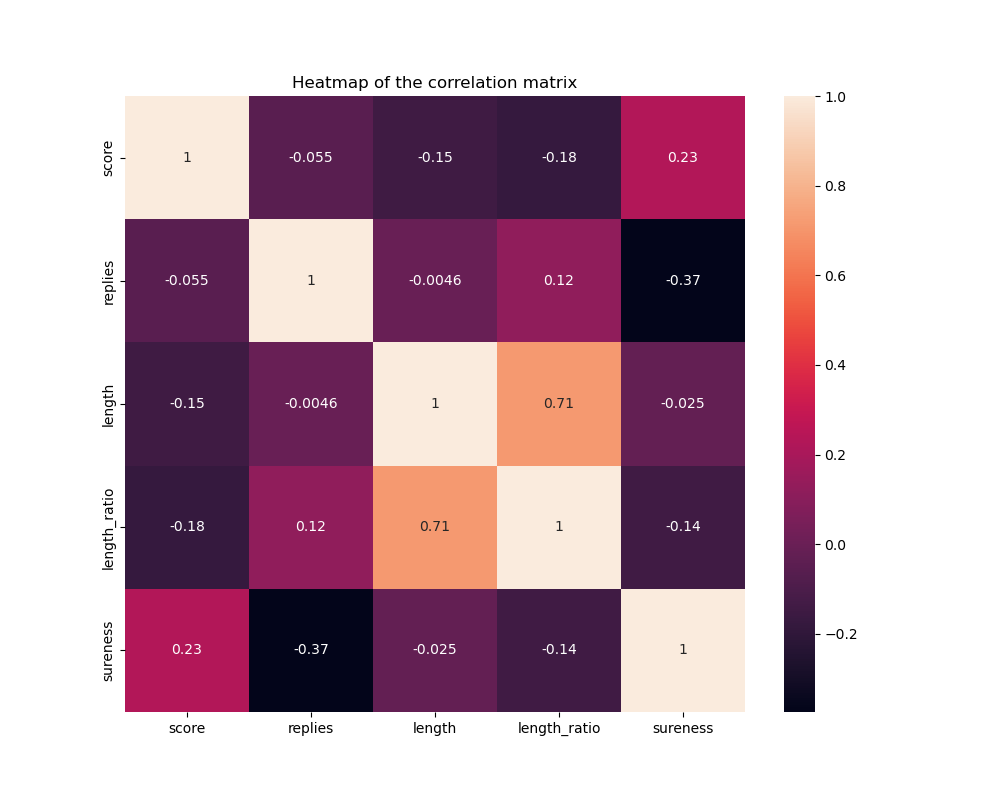
\includegraphics[width=\linewidth]{../plots/correlation_heatmap}
    \caption{Heatmap of correlation between different parameters (cues) of the data}
    \end{center}
\end{figure}


\section{Explainability}
Corresponds to points 4\&5 in the requirements.
\subsection{Problem Definition}
Explainability is the problem of different (usually were complex) machine learning models where the model works in a "black box" way. That is, the model learns a connection between the input and output features, however, it is unclear how this inference is made.\\

Some of the accepted ways of reducing the level of unexplainability include:\\
1. Visualizations of the output vectors provided by the model at each stage of its training. This helps in uderstanding how the clusters of models decisions change through time.\\
2. Training simpler and explainable (e.g. Decision Trees) models that learn to approximate the behaviour of the compelex and unexplainable one. Looking at the decision rules of the simpler model may help to understand the behavior of the complex one.\\
3. Feature Importance and Counterfactual methods are used to understand which features influence the models output the most, and conversely, small changes in which features lead to the biggest change in the model's prediction. This might help to glimpse the hidded connections between input and output features learned by the model.\\
4. Prototype and Criticism Based Methods are used to find which examples are thought by the model to be most representative of each class, and which are the most overlooked ones. This might help to understand the semantic representations learned by the model.

\subsection{Metacognition in Explainability}
In tasks of sureness prediction, metacognition may be crucial to understaning how the labels for each data-point were created.\\

Because machine learning models are trained to infer the label given the data, they are learning to approximate the connection between them.\\
Understanding metacognition may help us to understand how the humans have produced the labels, and therefore the possible connection that the model may have found. Furthermore, understanding the process underlying label creation in humans may help us to notice biases present in the training set, which would help to explain the biases expressed in the final model.

\subsection{Properties that help Explainability}
This project is very different from anything we have seen previously in the course. Mostly due to the fact that the judgement is approximated by other people (and not the one making the comment), and is made after the fact. (At a point when each comment was already seen and rated by the community.)\\
However, we try to find connections between our cues and the material we have learned.\\

As we have said earlier, in our data we have only 4 possible cues to the sureness, and we regard each of them below:
\begin{itemize}
    \item Score: we are not sure what we can connect this to, as this value is not based on some scale and only vaguely holds that "more is better" (but not always so). We do think, however, that it might be connected somewhat to the Hindsight Bias (lecture 7, pages 19+). We were asking our friends to grade the sureness of the person who wrote the answer before any score was given. So in some sense this is similar to what we have seen in class - someone who gets a bigger score would be graded in hindsight as being more sure than someone with a smaller score.
    \item Replies: we do not know exactly how to connect this to anything we have seen in class. As there are no immediate parallels.
    \item Length \& Length Ratio: we may be stretching it a little, but if we assume that correct answer is necessarily also concise - and therefore longer answer may be associated with being less sure. We could connect this cue to the relationship between hardness of the task and the time spend solving it (in general lecture 6. Specifically slides 13,14,15.) As more words written also require more time to write. 
\end{itemize}

\section{Use of BEVoCI Methodology}
Corresponds to points 6\&7 in the requirements.\\

First of all, we want to point out that in our case there is no "examinee".\\
Linear Mixed effects models (which are the basis for the Hierarchical Linear Regression, which are in terms the basis for nlme library in R and therefore for BEVoCI) account for the possiblity of dependent data points, which are a result of the same person responding to different questions (or same questions across time). They do so by introducing a group (or person)-based random effects.\\

In our case, and due to the fact that our data is a combination of 5 different people (otherwise we would not be able to train a deep learning model), "examinee" approach would not make sense.\\
\subsection{BEVoCI for Explainability of Neural Network}\label{sec:ffn_hlr}
If we looked solely on the performance on each of the models, we would have chosen to work with the KNN model, and we are not sure (conceptually) how the use of BEVoCI methodology would help in this case. Therefore, and due to the fact that we believe that applying BEVoCI to Neural Networks was the purpose of this project, we have chosen to do the BEVoCI analysis of the \hyperref[sec:ffn]{Feed Forward Neural Network} predictions.\\

In order to use the BEVoCI model to try and understand the cues that our neural network (\hyperref[sec:ffn]{Feed Forward Neural Network}) has used to make its predictions, we have trained the model on all of the available points (50), and made predictions on all of the same points. We have than saved this data into a new file (ffn\_data) upon which we have run Hirarchical Regression.\\

Contrary to the R language, python does not have a native implementation of the lme (Linear Mixed Effects) models.
Therefore (instead of implementing everything by hand), we have found a user-made implementation (HLR python library), and we express a deep gratitude to its creator. (Link to the github repository with the code - \href{https://github.com/teanijarv/HLR}{link}.)\\
We have selectively checked the code to make sure that it does what it is supposed to, and the creator himself writes that he checked many of the results against a code produced by a specialized library in SPSS.

In addition to the standard implementation of the Hirarchical Linear Regression, this library also calculates the F value, $R^2$, partial correlations, MSE and unique variance explained by each additional variable.\\
This library also includes the following statistical tests for each individual regression:
\begin{itemize}\label{list:stat_tests}
    \item \textbf{Independence of residuals (Durbin-Watson test)} - test for autocorrelation in the residuals from a statistical model or regression analysis. The Durbin-Watson statistic will always have a value ranging between 0 and 4. A value of 2.0 indicates there is no autocorrelation detected in the sample. Values from 0 to less than 2 point to positive autocorrelation, and values from 2 to 4 mean negative autocorrelation. (\href{https://www.investopedia.com/terms/d/durbin-watson-statistic.asp#:~:text=The%20Durbin%20Watson%20(DW)%20statistic,autocorrelation%20detected%20in%20the%20sample.}{Source})
    \item \textbf{Linearity (Pearson r)} - a correlation coefficient that measures linear correlation between two sets of data. It is the ratio between the covariance of two variables and the product of their standard deviations. (\href{https://en.wikipedia.org/wiki/Pearson_correlation_coefficient}{Source})
    \item \textbf{Linearity (Rainbow test)} - even if the true relationship is non-linear, a good linear fit can be achieved on a subsample in the "middle" of the data. The null hypothesis is rejected whenever the overall fit is significantly worse than the fit for the subsample. (\href{https://search.r-project.org/CRAN/refmans/lmtest/html/raintest.html}{Source})
    \item \textbf{Homoscedasticity (Breusch-Pagan test)} - tests whether the variance of the errors from a regression is dependent on the values of the independent variables (in this case there is heteroskedasticity). (\href{https://en.wikipedia.org/wiki/Breusch%E2%80%93Pagan_test}{Source})
    \item \textbf{Homoscedasticity (Goldfeld-Quandt test)} - used to test the presence of Heteroscedasticity in the given data. It does so by splitting the data into two sets with respect to a single chosen variable, and compares the residuals in the two sets. (Can miss heteroskedasticity if the split is done w.r.t a variable that does not have heteroskedasticity.) (\href{https://www.geeksforgeeks.org/goldfeld-quandt-test/}{Source 1}, \href{https://stats.stackexchange.com/questions/468778/contradictory-results-between-breusch-pagan-test-and-goldfeld-quandt-test-in-pyt}{Source 2}, \href{https://en.wikipedia.org/wiki/Goldfeld%E2%80%93Quandt_test}{Source 3})
    \item \textbf{Multicollinearity (pairwise correlations)} - checks for a situation where (some of) the predictors in a regression model are linearly dependent. (But only pariwise correlations.)
    \item \textbf{Multicollinearity (Variance Inflation Factors)} - measures the multicollinearity between the predictors by looking at the ratio (quotient) of the variance of a parameter estimate when fitting a full model that includes other parameters to the variance of the parameter estimate if the model is fit with only the parameter on its own. (\href{https://en.wikipedia.org/wiki/Variance_inflation_factor}{Source})
    \item \textbf{Outliers (extreme standardized residuals)} - checks for unusual outliers by looking at the extremely high or low (higher than 3 or lower than -3) values of the residuals. (\href{https://www.statisticshowto.com/what-is-a-standardized-residuals/#:~:text=If%20your%20residuals%20are%20%2B%2F%2D,standard%20deviations%20from%20the%20mean.}{Source})
    \item \textbf{Outliers (high Cooks distance)} - tries to detect outliers by looking at the Cook’s distance. It is a measure of the effect of deleting an observation on the estimated coefficients. It takes into account both the leverage and the residual of the observation. High Cook’s distance indicates that the observation has a large effect on the estimated coefficients when it’s deleted. (\href{https://prepnuggets.com/glossary/cooks-distance/#:~:text=Cook's%20distance%20is%20a%20measure,estimated%20coefficients%20when%20it's%20deleted.}{Source})
    \item \textbf{Normality (mean of residuals)} - checks for the assumption of normality of residuals by looking at their mean. (Normality assumption holds if the mean is around 0.)
    \item \textbf{Normality (Shapiro-Wilk test)} - specific numerical test to check the residual normality assumption. (\href{https://en.wikipedia.org/wiki/Shapiro%E2%80%93Wilk_test}{Source})
\end{itemize}

Many of these tests were unknown to us previous to encountering them in this library, so we cannot say that we fully understand either the tests themselves, or their implications; but we have chosen to include their results in any case for a more knowledged reader to interpret.

Additionally, we would like to point out that we have not encountered the concept of Hierarchical Regression Models before this projects, therefore we in no way claim deep understanding and/or proficiency in the use of these models. Therefore, some of our conclusions might be invalid or simply wrong, however, this is due to inexperience but not malice.\\

We have tried the following hierarchies:\\
(In each model the dependent variable is 'sureness' and we list the independent variables we have used for the regression.)\\

\textbf{Hierarchy 1}
\begin{itemize}
    \item score
    \item score, replies
    \item score, replies, length
    \item score, replies, length, length ratio
\end{itemize}

\textbf{Hierarchy 2}
\begin{itemize}
    \item score
    \item score, replies
    \item score, replies, length ratio
\end{itemize}

\textbf{Hierarchy 3}
\begin{itemize}
    \item score
    \item score, length
\end{itemize}

\textbf{Hierarchy 4}
\begin{itemize}
    \item score
    \item score, length ratio
\end{itemize}

\textbf{Hierarchy 5}
\begin{itemize}
    \item replies
    \item replies, length
\end{itemize}

\textbf{Hierarchy 6}
\begin{itemize}
    \item replies
    \item replies, length ratio
\end{itemize}

\textbf{Hierarchy 7}
\begin{itemize}
    \item length
    \item length, length ratio
\end{itemize}

\textbf{Hierarchy 8}
\begin{itemize}
    \item replies
    \item replies, score
    \item replies, score, length ratio
\end{itemize}

In all of the hierarchies (except for the first one, just to see what would happen) we have included either the length or the length ratio, but never both. They have a very high correlation, and therefore do not pass the rule of thumb presented in the BEVoCI paper, which is to include a cue only of correlation is less than 0.3. For that matter, models which include both cues also do not pass the multicollinearity tests.

By looking at the statistical results over for all of the hierarchies, we can come to a few conclusions:
\begin{itemize}
    \item No combination of cues is valid enough to use Linear Regression at all. Plausibly, this is due to the fact that many of the tests checking for the assumptions of linear regression fail for most of the cues.
    \item In general, it seems that the informative content (higher $R^2$ and lower p-value for validness of regression) is ordered as follows: score $>$ replies $>$ length $>$ length ratio
    \end{itemize}

Therefore, we present here the statistical results only for the most informative model/hierarchy - hierarchy 1 with the cues: score, replies, length. However, the complete results (including all of the corresponding graphs) can be found in the 'data\_exploration.ipynb' file, or in the pdf export which we include with this file.\\

Here is a table of (selected) statistical results for hierarchy 1:
\begin{table}[H]
  \begin{center}
  \begin{tabular}{|l|c|c|c|}
    \hline
    cues & $R^2$ & F-value & p-value (F) \\
    \hline
    score & 0.0562 & 2.8582 & 0.0974 \\
    score, replies & 0.101 & 2.6282 & 0.0828  \\
    score, replies, length & 0.1276 & 2.2428 & 0.096  \\
    \hline
  \end{tabular}
  \caption{Statistical Results for Hiearachy 1 - part 1}
  \end{center}
\end{table}

\begin{table}[H]
  \begin{center}
  \begin{tabular}{|l|c|c|}
    \hline
    cues & coefs (const; cues) & p-value coefs (const; cues) \\
    \hline
    score & 76.36; -0.0037 & 0; 0.0974 \\
    score, replies & 76.68; -0.0039; -0.1295 & 0; 0.08; 0.13 \\
    score, replies, length & 77.24; -0.0043; -0.13; -0.0044 & 0; 0.056; 0.13; 0.24 \\
    \hline
  \end{tabular}
  \caption{Statistical Results for Hiearachy 1 - part 2}
  \end{center}
\end{table}

\begin{table}[H]
  \begin{center}
  \begin{tabular}{|l|c|c|c|c|}
    \hline
    cues & semi-partial corrs. & $R^2$ change & F-value change & p-value (F change) \\
    \hline
    score & -0.24 & - & - & - \\
    score, replies & -0.25; -0.21 & 0.044 & 2.32 & 0.13 \\
    score, replies, length & -0.27; -0.21; -0.16 & 0.027 & 1.42 & 0.24 \\
    \hline
  \end{tabular}
  \caption{Statistical Results for Hiearachy 1 - part 3}
  \end{center}
\end{table}

Here are the results from the statistical tests (in the same order in which we have presented them earlier - \hyperref[list:stat_tests]{Statistical Tests}) (test result, p-value (if relevant)):
\begin{table}[H]
  \begin{center}
  \begin{tabular}{|l|c|c|c|c|c|c|}
    \hline
    cues & DW & Pearson r & Rainbow & BP & GQ & Pairwise \\
    \hline
    score & T & \textcolor{red}{(F, 0.097)} & (T, 0.39) & (T, 0.64) & (T, 0.91) & T \\
    score, replies & T & \textcolor{red}{=; (F, 0.17)} & (T, 0.25) & (T, 0.67) & (T, 0.94) & T \\
    score, replies, length & T & \textcolor{red}{=; =; (F, 0.39)} & (T, 0.25) & (T, 0.47) & (T, 0.94) & T \\
    \hline
  \end{tabular}
  \caption{Statistical Tests for Hierarchy 1 - part 1}
  \end{center}
\end{table}

\begin{table}[H]
  \begin{center}
  \begin{tabular}{|l|c|c|c|c|c|c|}
    \hline
    cues & VIF & Extreme Residuals & Cooks & Mean Residuals & SW \\
    \hline
    score  & T & T & T & T & \textcolor{red}{(F, 0.006)} \\
    score, replies & T & T & T & T & \textcolor{red}{(F, 0.004)} \\
    score, replies, length & T & T & T & T & \textcolor{red}{(F, 0.009)} \\
    \hline
  \end{tabular}
  \caption{Statistical Tests for Hierarchy 1 - part 2}
  \end{center}
\end{table}

Plots of the graphs of different statistical values:
\begin{figure}[H]
\centering
\begin{subfigure}{.5\textwidth}
  \centering
  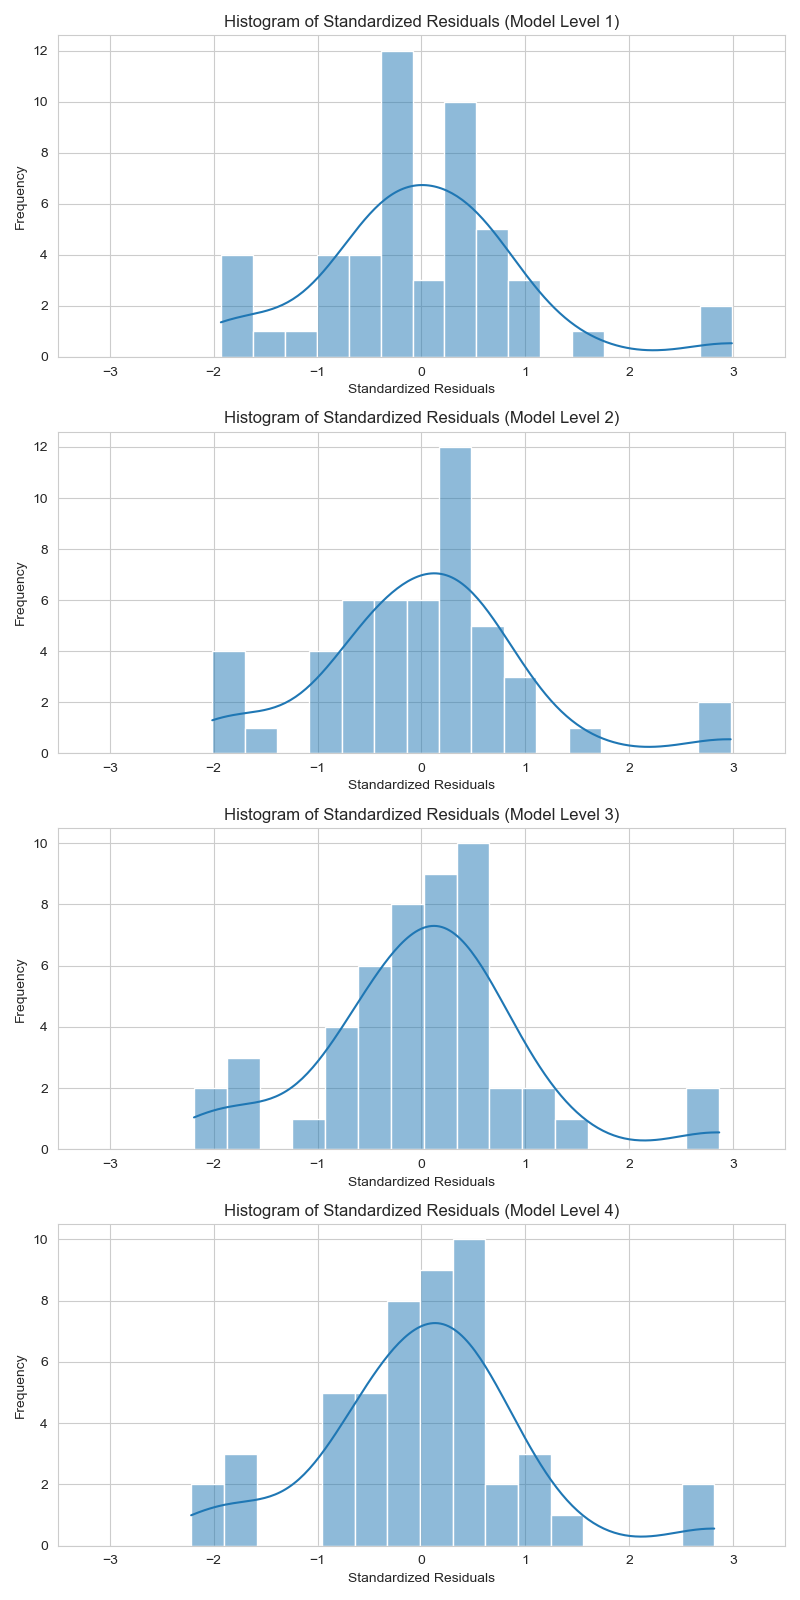
\includegraphics[width=\linewidth]{../plots/fnn_data/hierarchy1/histogram_std_residuals}
  \caption{Standardized Residuals Historgram}
\end{subfigure}%
\begin{subfigure}{.5\textwidth}
  \centering
  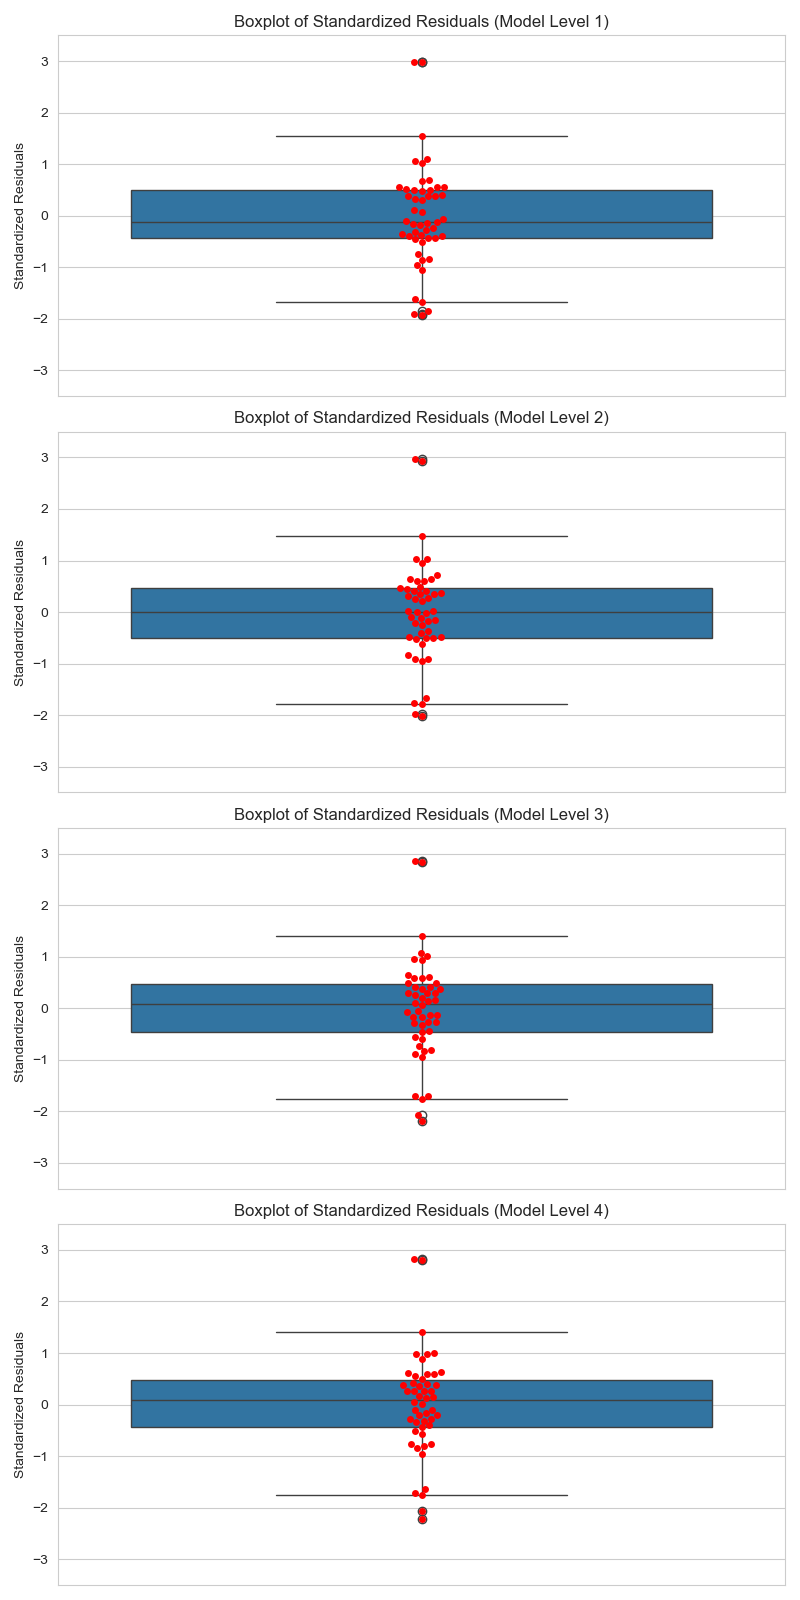
\includegraphics[width=\linewidth]{../plots/fnn_data/hierarchy1/std_residuals}
  \caption{Boxplot of Standardized Residuals}
\end{subfigure}
\end{figure}

\begin{figure}[H]
\centering
\begin{subfigure}{.5\textwidth}
  \centering
  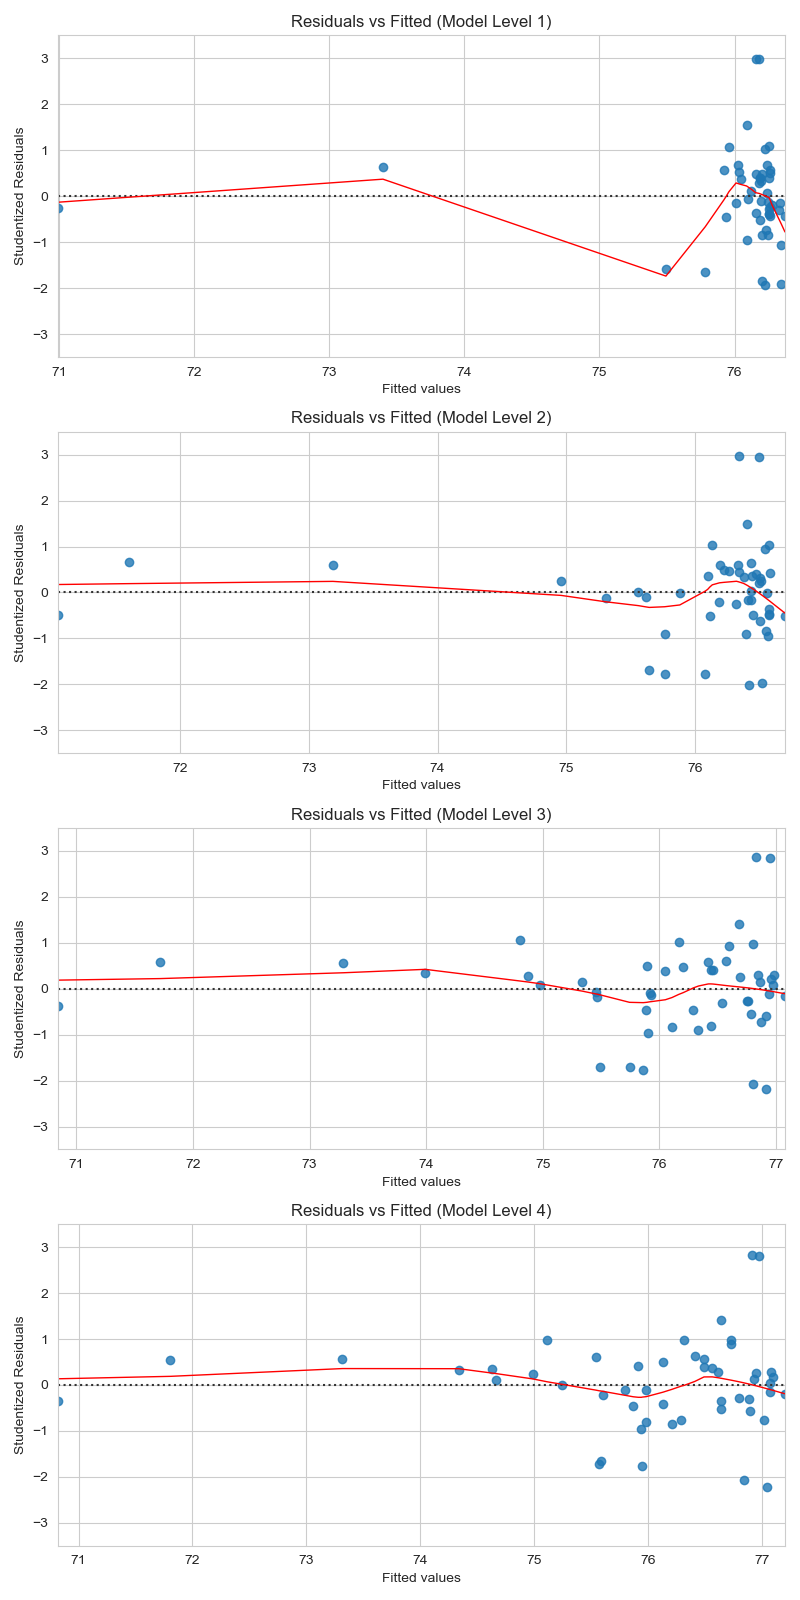
\includegraphics[width=\linewidth]{../plots/fnn_data/hierarchy1/studentized_residuals_vs_fitted}
  \caption{Standardized Residuals plot}
\end{subfigure}%
\begin{subfigure}{.5\textwidth}
  \centering  
  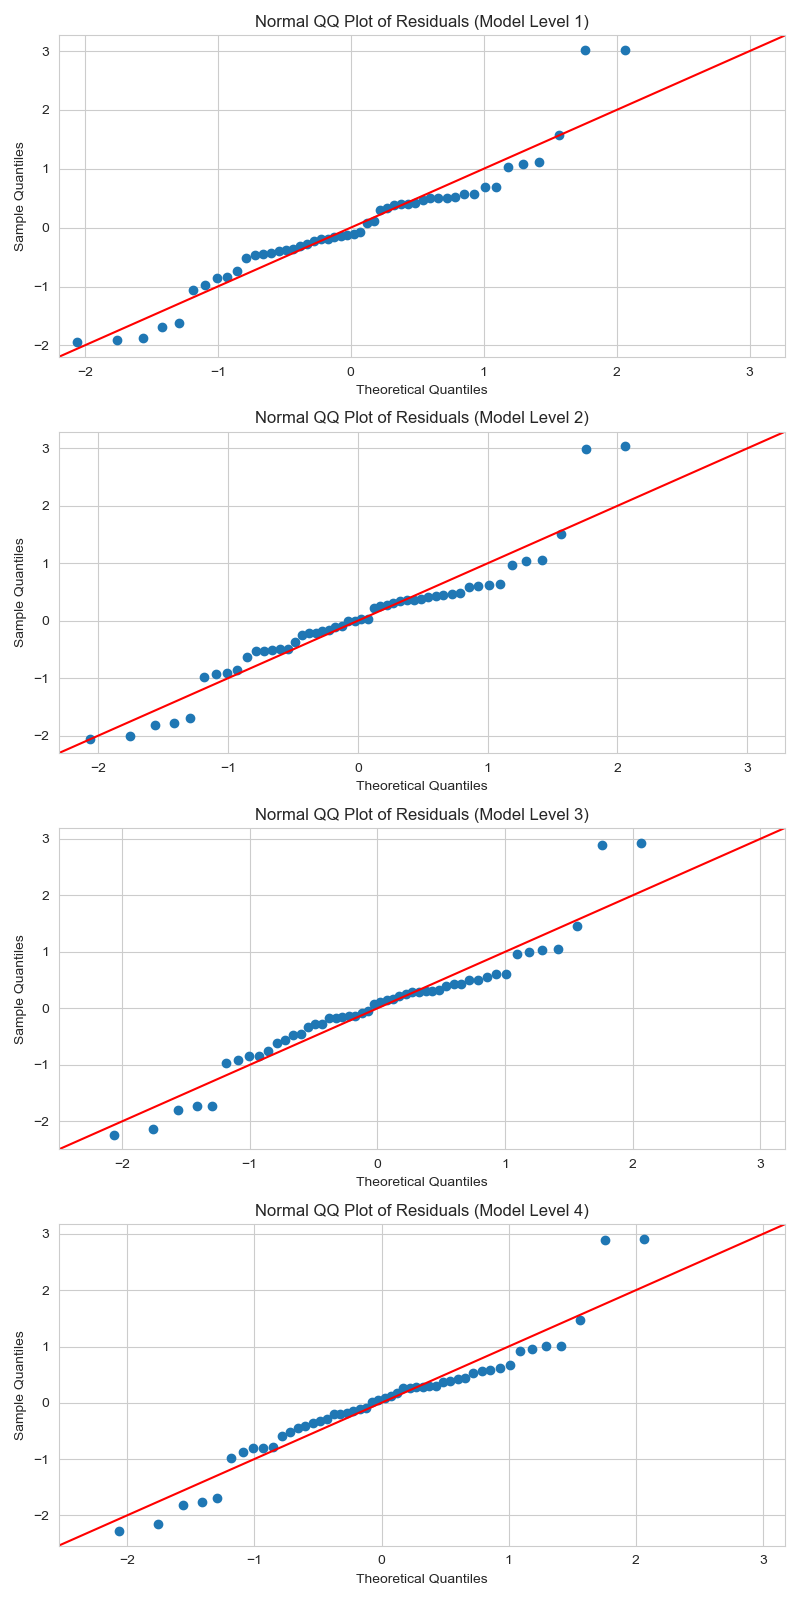
\includegraphics[width=\linewidth]{../plots/fnn_data/hierarchy1/qq_residuals}
  \caption{QQ plot of Standardized Residuals}
\end{subfigure}
\end{figure}

\begin{figure}[H]
    \begin{center}
    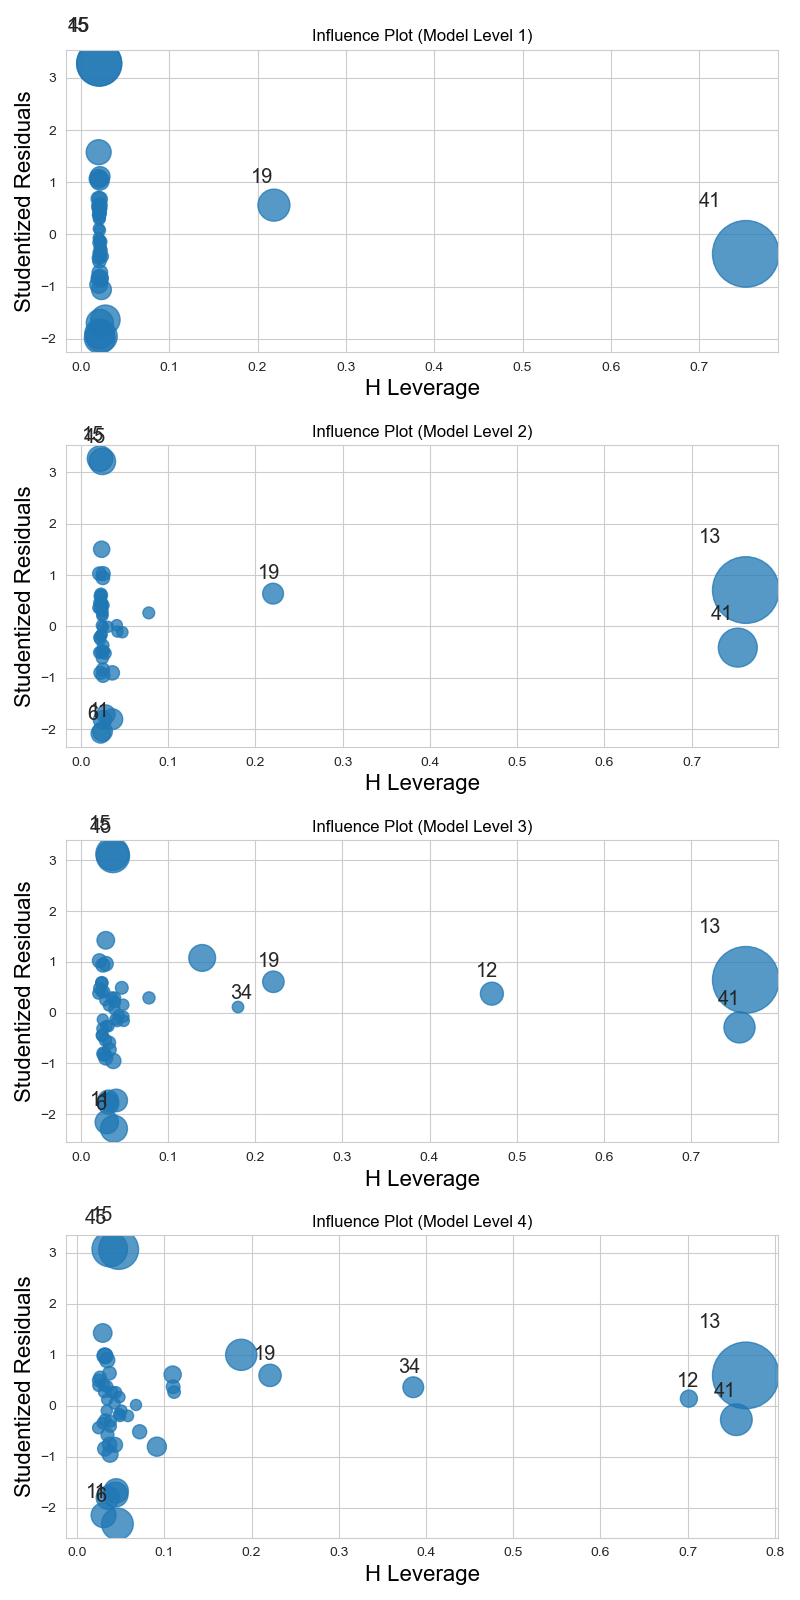
\includegraphics[width=0.5\linewidth]{../plots/fnn_data/hierarchy1/influence}
    \caption{Plot of influence of Different Points on the model}
    \end{center}
\end{figure}

\begin{figure}[H]
\centering
\begin{subfigure}{.5\textwidth}
  \centering
  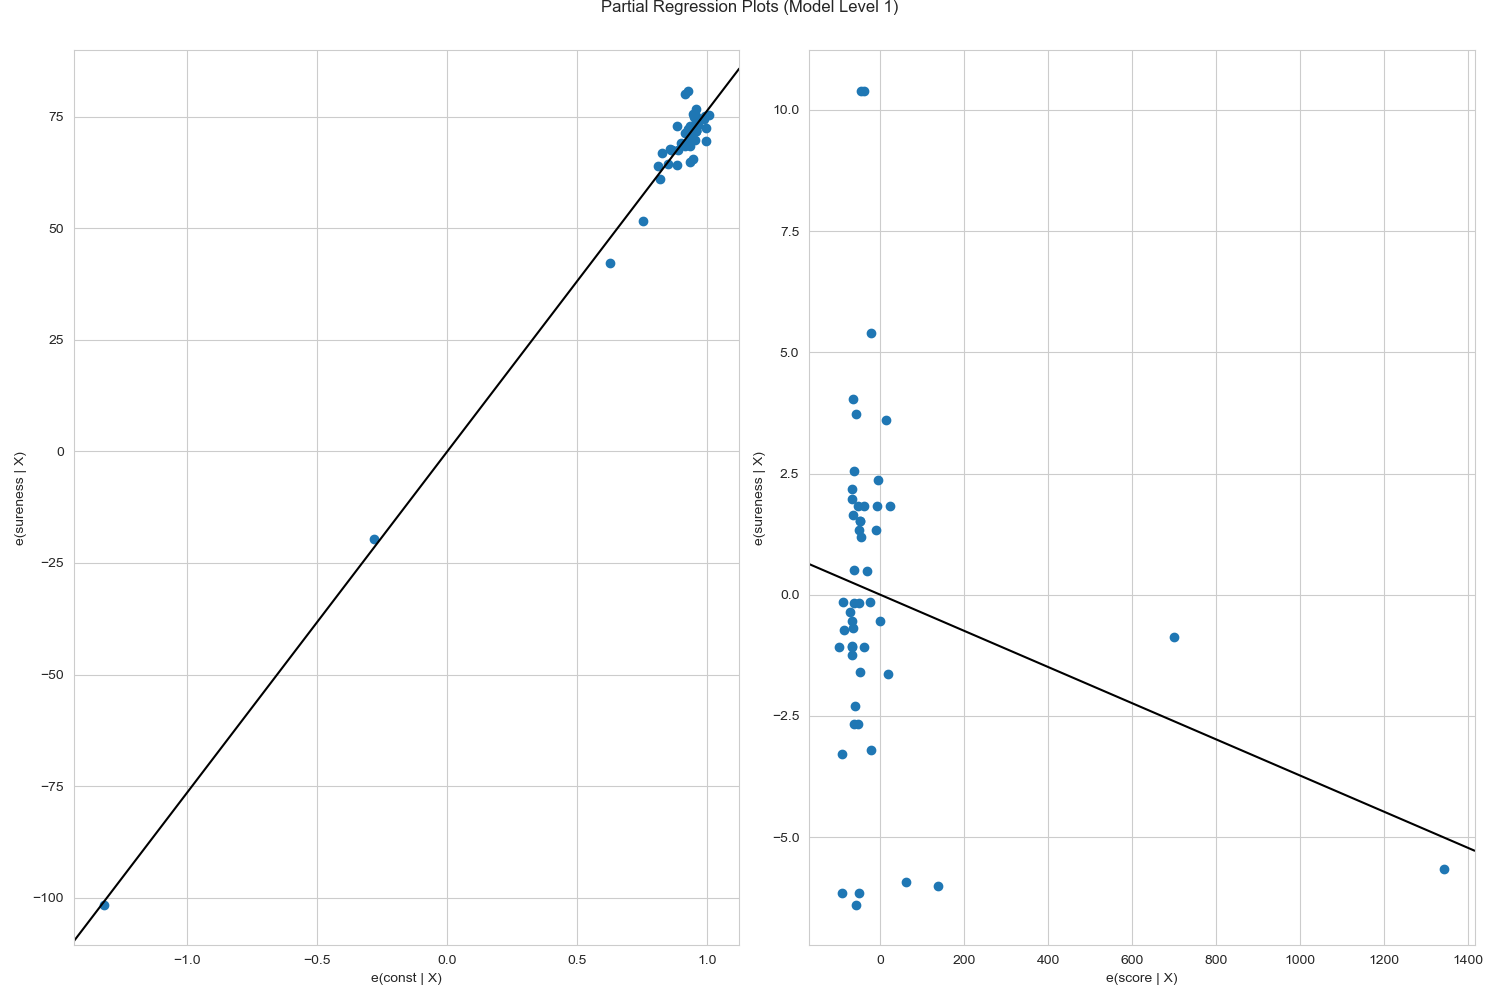
\includegraphics[width=\linewidth]{../plots/fnn_data/hierarchy1/partial_regression_0}
  \caption{score}
\end{subfigure}%
\begin{subfigure}{.5\textwidth}
  \centering
  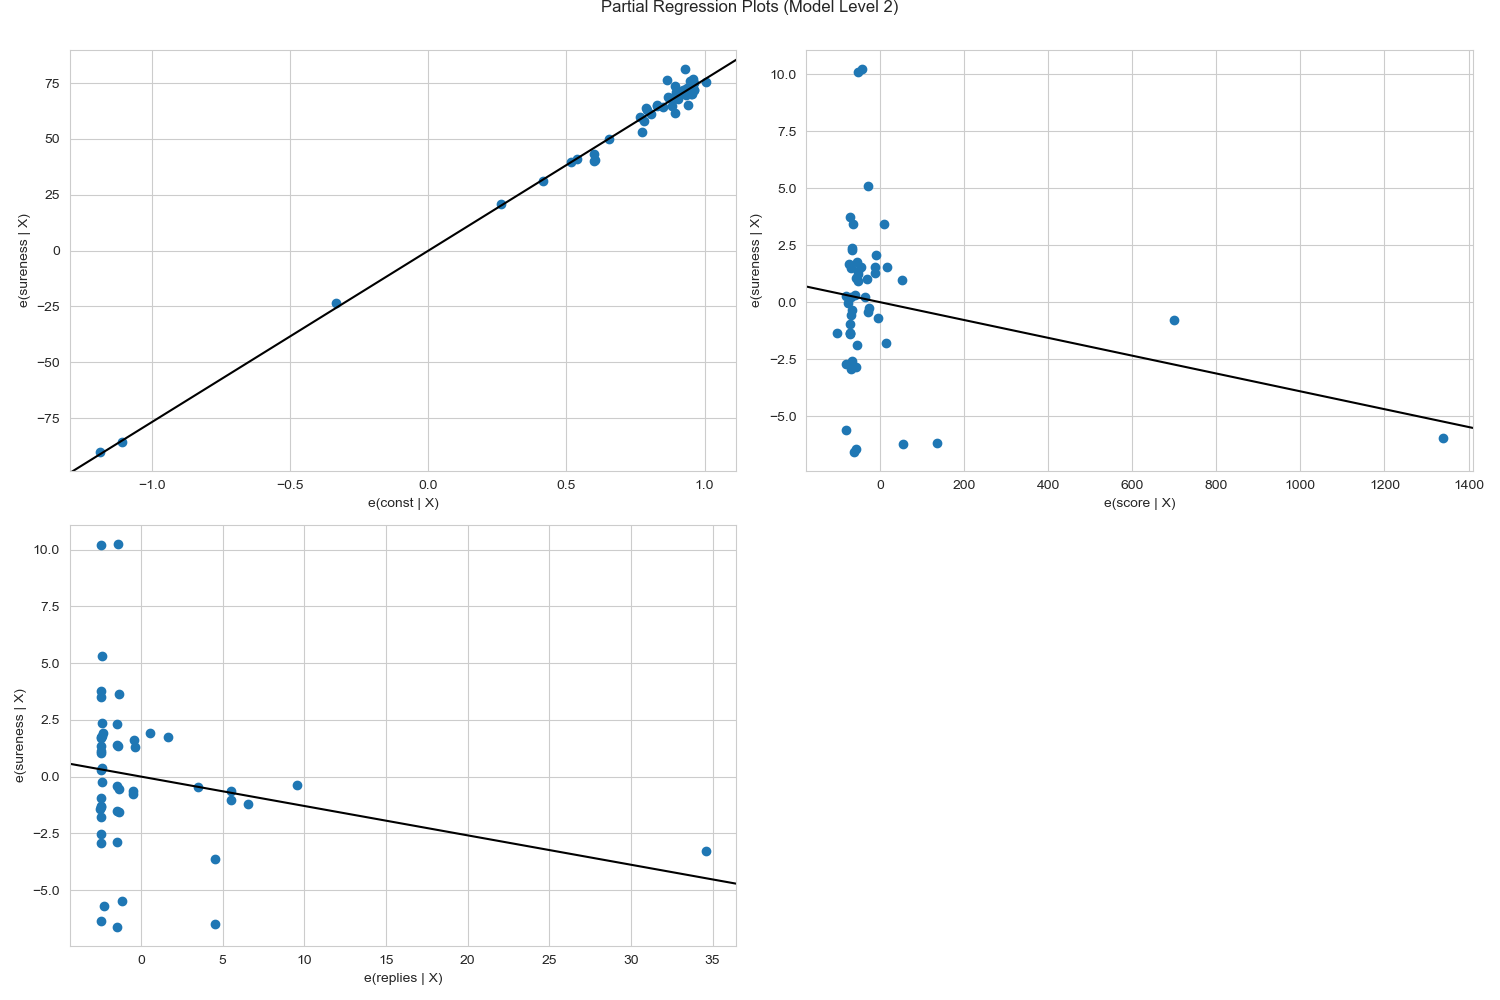
\includegraphics[width=\linewidth]{../plots/fnn_data/hierarchy1/partial_regression_1}
  \caption{score; replies}
\end{subfigure}
\begin{subfigure}{.5\textwidth}
  \centering
  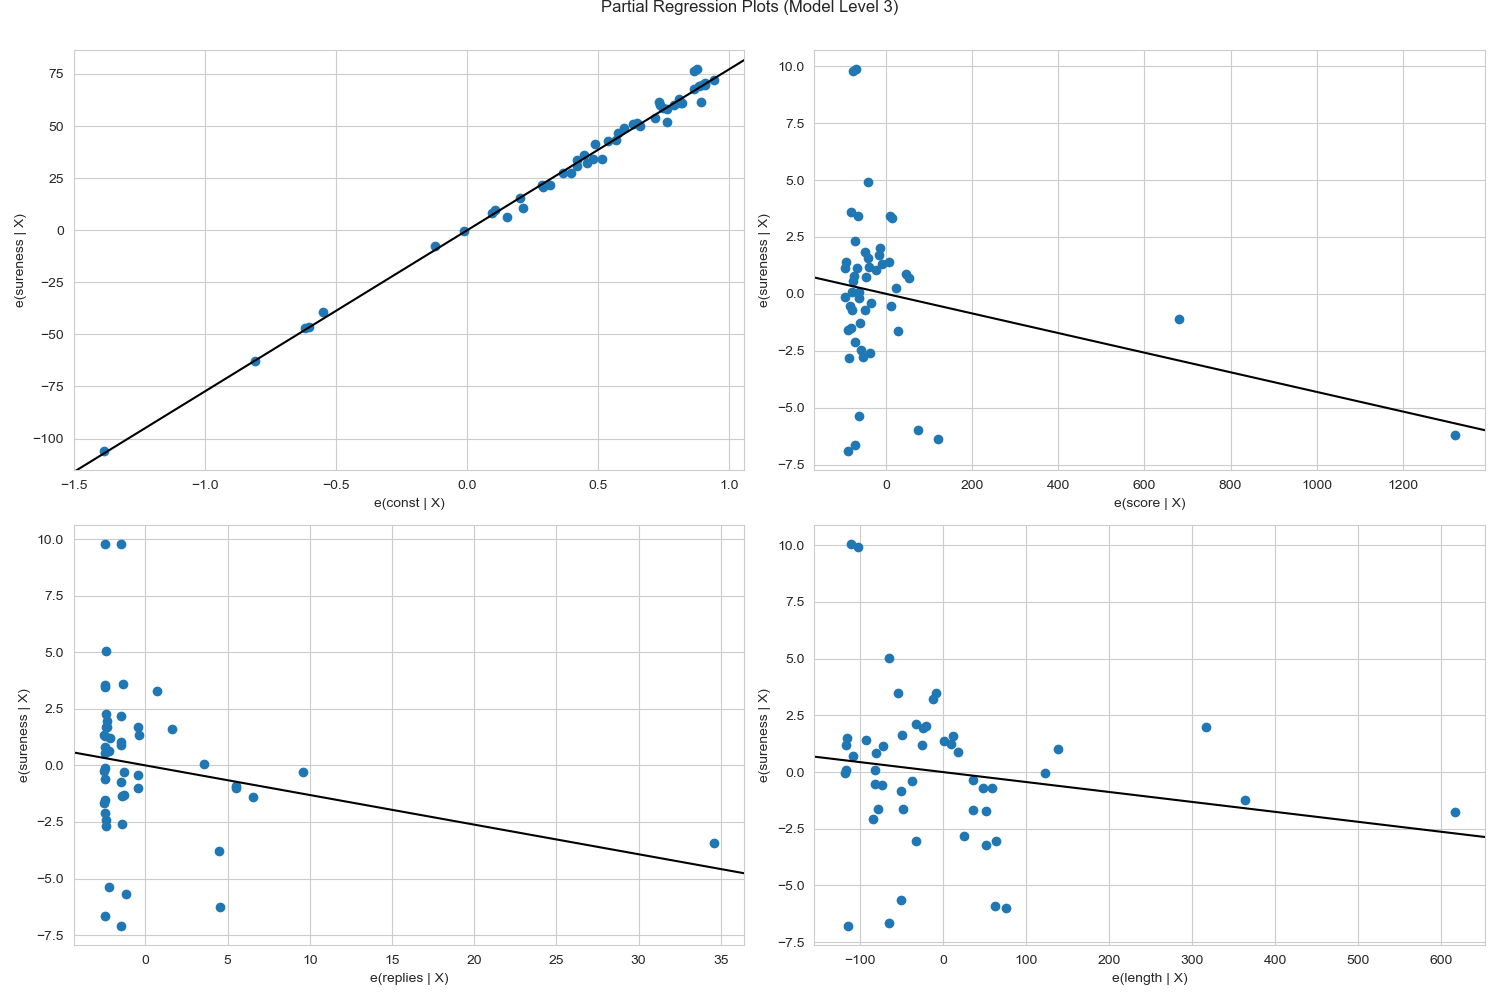
\includegraphics[width=\linewidth]{../plots/fnn_data/hierarchy1/partial_regression_2}
  \caption{score; replies; length}
\end{subfigure}%
\begin{subfigure}{.5\textwidth}
  \centering
  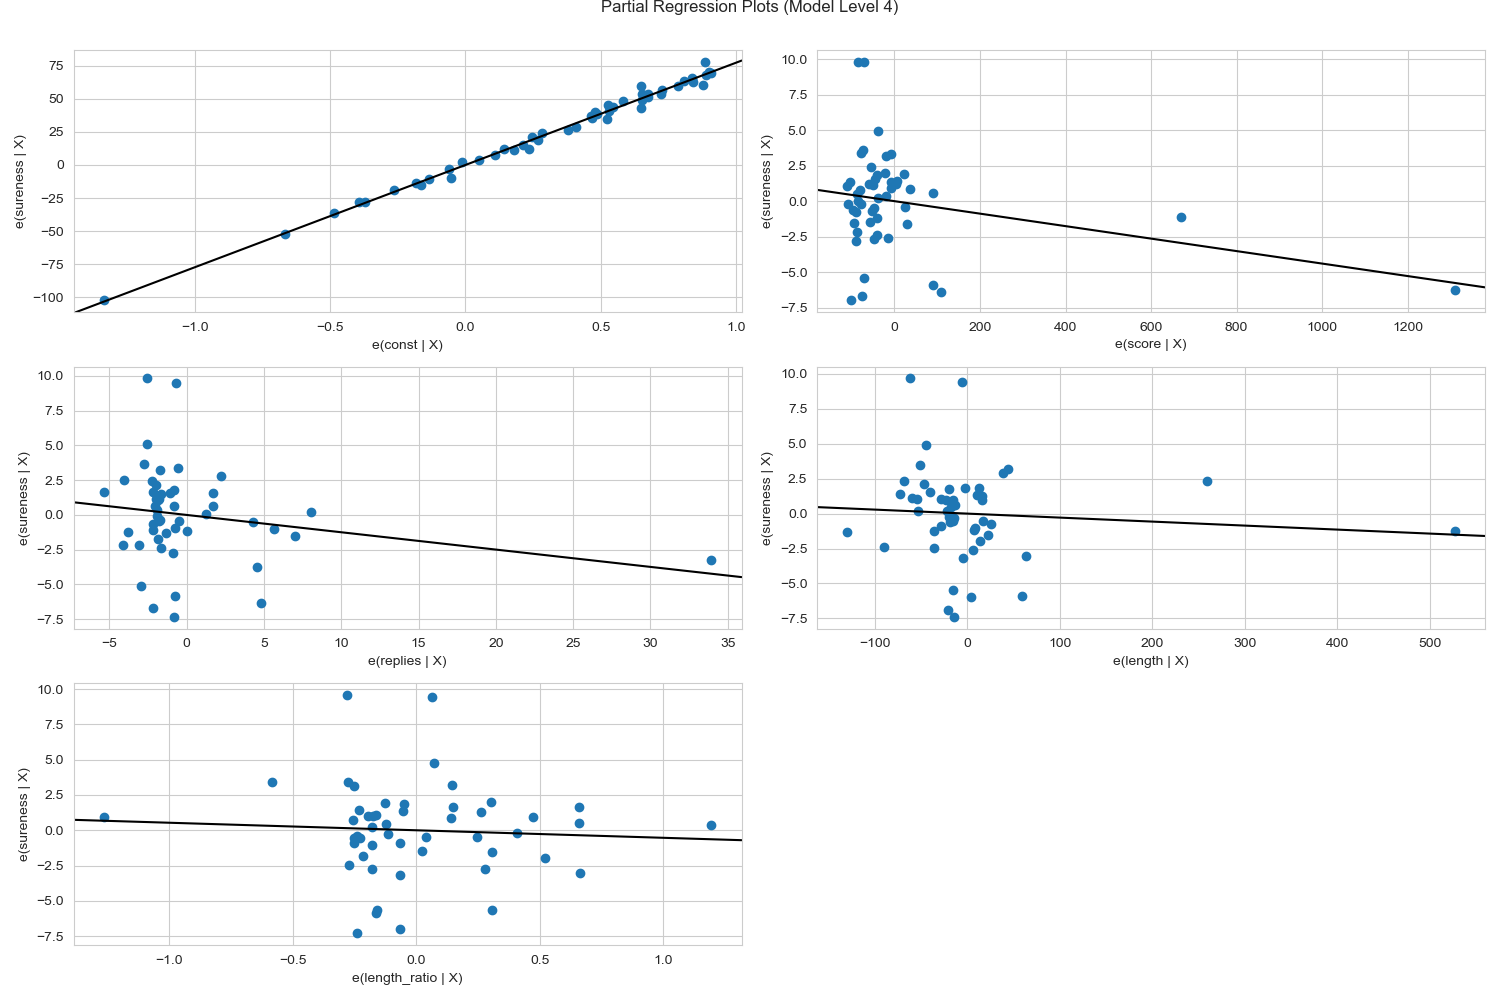
\includegraphics[width=\linewidth]{../plots/fnn_data/hierarchy1/partial_regression_3}
  \caption{score; replies; length; length ratio}
\end{subfigure}
\caption{Plots of Standardized Residuals as a function of each individual cue + constant}
\end{figure}

Plots of different cues and their effects on the final sureness:
\begin{figure}[H]
\centering
\begin{subfigure}{.5\textwidth}
  \centering
  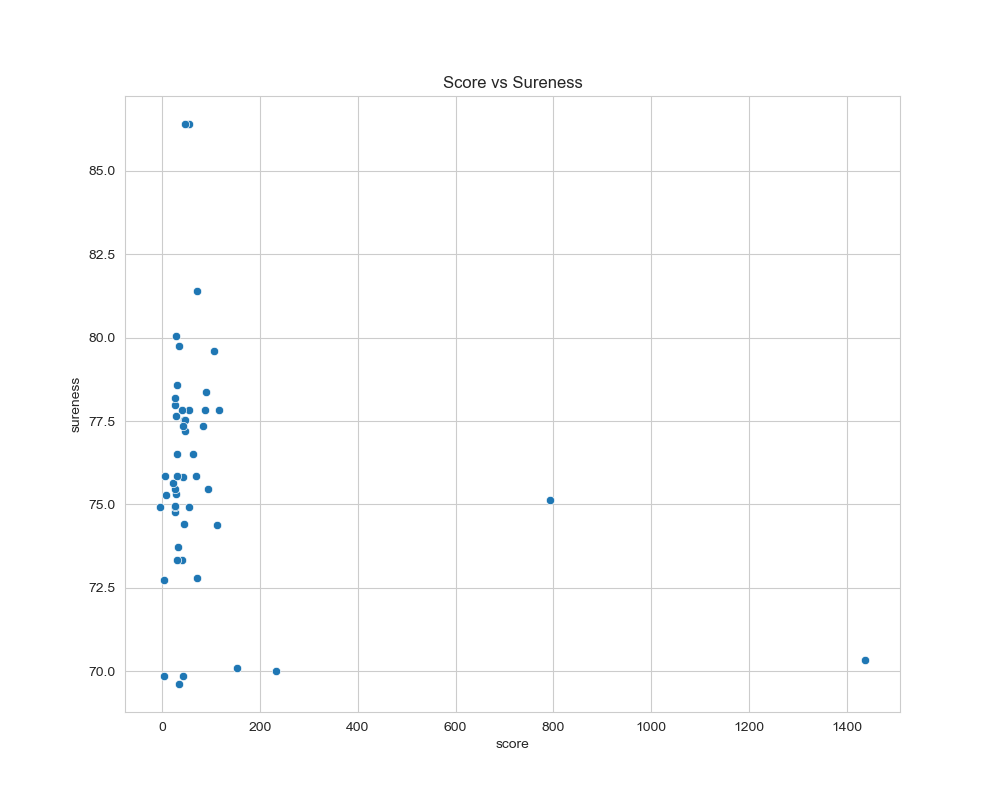
\includegraphics[width=\linewidth]{../plots/fnn_data/score_vs_sureness}
  \caption{Score - Sureness}
\end{subfigure}%
\begin{subfigure}{.5\textwidth}
  \centering
  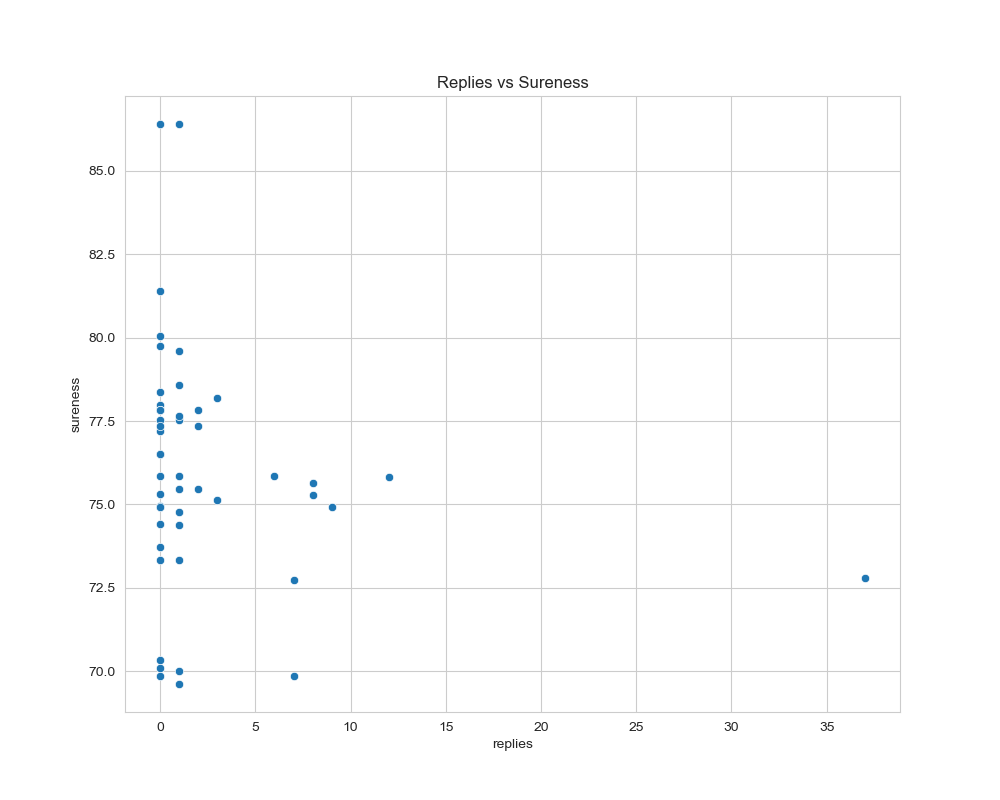
\includegraphics[width=\linewidth]{../plots/fnn_data/replies_vs_sureness}
  \caption{Replies - Sureness}
\end{subfigure}
\begin{subfigure}{.5\textwidth}
  \centering
  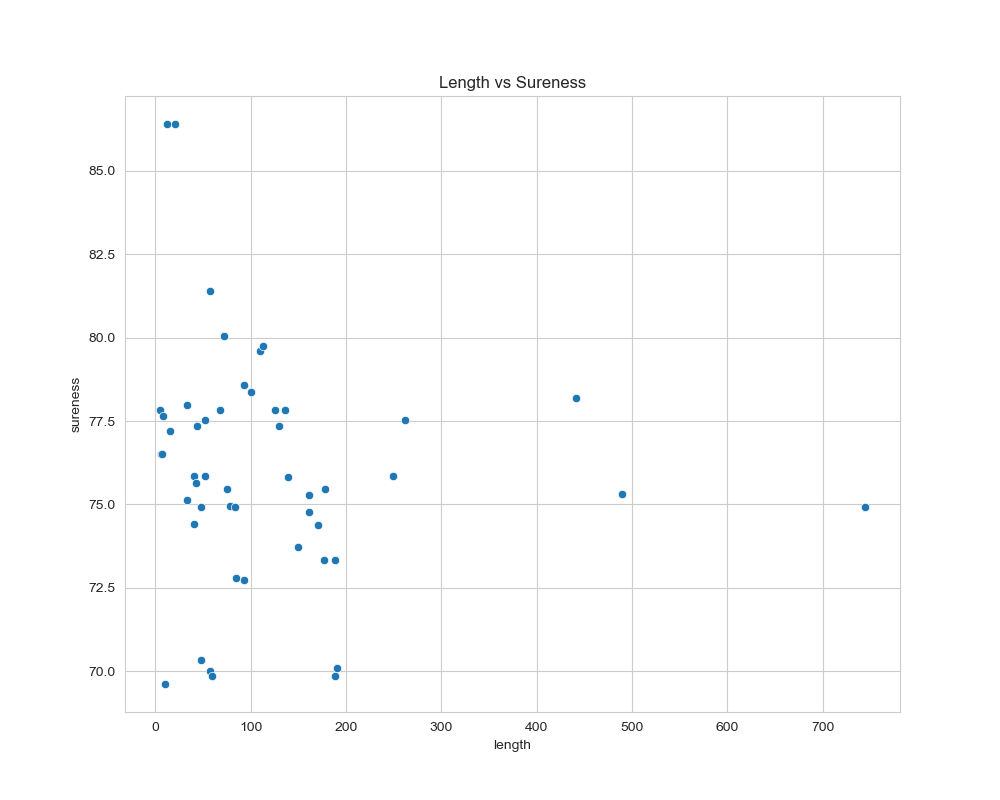
\includegraphics[width=\linewidth]{../plots/fnn_data/length_vs_sureness}
  \caption{Length - Sureness}
\end{subfigure}%
\begin{subfigure}{.5\textwidth}
  \centering
  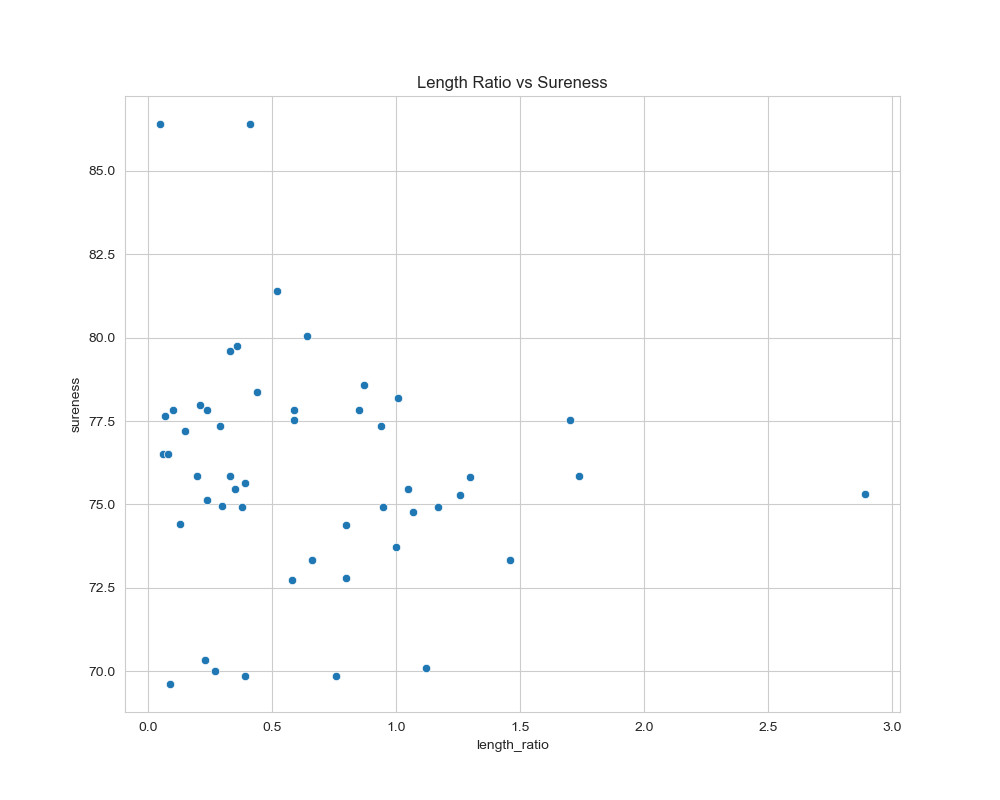
\includegraphics[width=\linewidth]{../plots/fnn_data/length_ratio_vs_sureness}
  \caption{Length Ratio - Sureness}
\end{subfigure}
\caption{Different Cues and their Effects on the final Sureness}
\end{figure}

\subsection{BEVoCI for Meta Cognition}\label{sec:mc_hlr}
After applying the BEVoCI methods to the data produced by the Feed Forward Neural Network, we were interested in applying the same method to the origianal data - this would help us understand if the performance of the neural network was so bad due to the small number of points, or rather due to the general lack of regularity in the data.\\
We have used here the same hierarchies, and the same statistical tests as we have done for Neural Network analysis.

In a similar way to the analysis of the Feed Forward Network, here we come to the following conclusions:
\begin{itemize}
    \item There is only one cue which makes use of Linear Regression valid - replies. (Other cues do not get this validity, plausibly due, again, to the fact that many of the tests checking for the assumptions of linear regression fail for them.)
    \item In general, it seems that the informative content (higher R2 and lower p-value for validness of regression) is ordered as follows: replies $>$ score $>$ length ratio $>$ length. (Notice that it is quite different from the results we got in \hyperref[sec:ffn_hlr]{BEVoCI for Meta Cognition}.)
\end{itemize}

Therefore, we present here the statistical results only for the most informative model/hierarchy - hierarchy 8 with the cues: replies, score, length ratio. However, the complete results (including all of the corresponding graphs) can be found in the 'data\_exploration.ipynb' file, or in the pdf export which we include with this file.\\

Here is a table of (selected) statistical results for hierarchy 8:
\begin{table}[H]
  \begin{center}
  \begin{tabular}{|l|c|c|c|}
    \hline
    cues & $R^2$ & F-value & p-value (F) \\
    \hline
    replies & 0.14 & 7.83 & 0.0074 \\
    replies, score & 0.184 & 5.3 & 0.0084  \\
    replies, score, length ratio & 0.1876 & 3.54 & 0.022  \\
    \hline
  \end{tabular}
  \caption{Statistical Results for Hiearachy 1 - part 1}
  \end{center}
\end{table}

\begin{table}[H]
  \begin{center}
  \begin{tabular}{|l|c|c|}
    \hline
    cues & coefs (const; cues) & p-value coefs (const; cues) \\
    \hline
    replies & 78.17; -0.578 & 0; 0.0074 \\
    replies, score & 77.35; -0.56; 0.0083 & 0; 0.0084; 0.12 \\
    replies, score, length ratio & 78; -0.55; 0.0079; -0.99 & 0; 0.011; 0.15; 0.66 \\
    \hline
  \end{tabular}
  \caption{Statistical Results for Hiearachy 1 - part 2}
  \end{center}
\end{table}

\begin{table}[H]
  \begin{center}
  \begin{tabular}{|l|c|c|c|c|}
    \hline
    cues & semi-partial corrs. & $R^2$ change & F-value change & p-value (F change) \\
    \hline
    replies & -0.374 & - & - & - \\
    replies, score & -0.36; 0.21 & 0.044 & 2.52 & 0.12 \\
    replies, score, length ratio & -0.35; 0.2; -0.06 & 0.0036 & 0.2 & 0.65 \\
    \hline
  \end{tabular}
  \caption{Statistical Results for Hiearachy 1 - part 3}
  \end{center}
\end{table}

Here are the results from the statistical tests (in the same order in which we have presented them earlier - \hyperref[list:stat_tests]{Statistical Tests}) (test result, p-value (if relevant)):
\begin{table}[H]
  \begin{center}
  \begin{tabular}{|l|c|c|c|c|c|c|}
    \hline
    cues & DW & Pearson r & Rainbow & BP & GQ & Pairwise \\
    \hline
    replies & T & \textcolor{ForestGreen}{(T, 0.0074)} & (T, 0.79) & (T, 0.7) & (T, 0.85) & T \\
    replies, score & T & \textcolor{red}{=; (F, 0.11)} & (T, 0.75) & (T, 0.83) & (T, 0.73) & T \\
    replies, score, length ratio & T & \textcolor{red}{=; =; (F, 0.33)} & (T, 0.71) & (T, 0.9) & (T, 0.5) & T \\
    \hline
  \end{tabular}
  \caption{Statistical Tests for Hierarchy 1 - part 1}
  \end{center}
\end{table}

\begin{table}[H]
  \begin{center}
  \begin{tabular}{|l|c|c|c|c|c|c|}
    \hline
    cues & VIF & Extreme Residuals & Cooks & Mean Residuals & SW \\
    \hline
    replies  & T & T & \textcolor{red}F & T & \textcolor{ForestGreen}{(T, 0.11)} \\
    replies, score & T & T & \textcolor{red}F & T & \textcolor{ForestGreen}{(T, 0.16)} \\
    replies, score, length ratio & T & T & \textcolor{red}F & T & \textcolor{ForestGreen}{(T, 0.1)} \\
    \hline
  \end{tabular}
  \caption{Statistical Tests for Hierarchy 1 - part 2}
  \end{center}
\end{table}

Plots of the graphs of different statistical values:
\begin{figure}[H]
\centering
\begin{subfigure}{.5\textwidth}
  \centering
  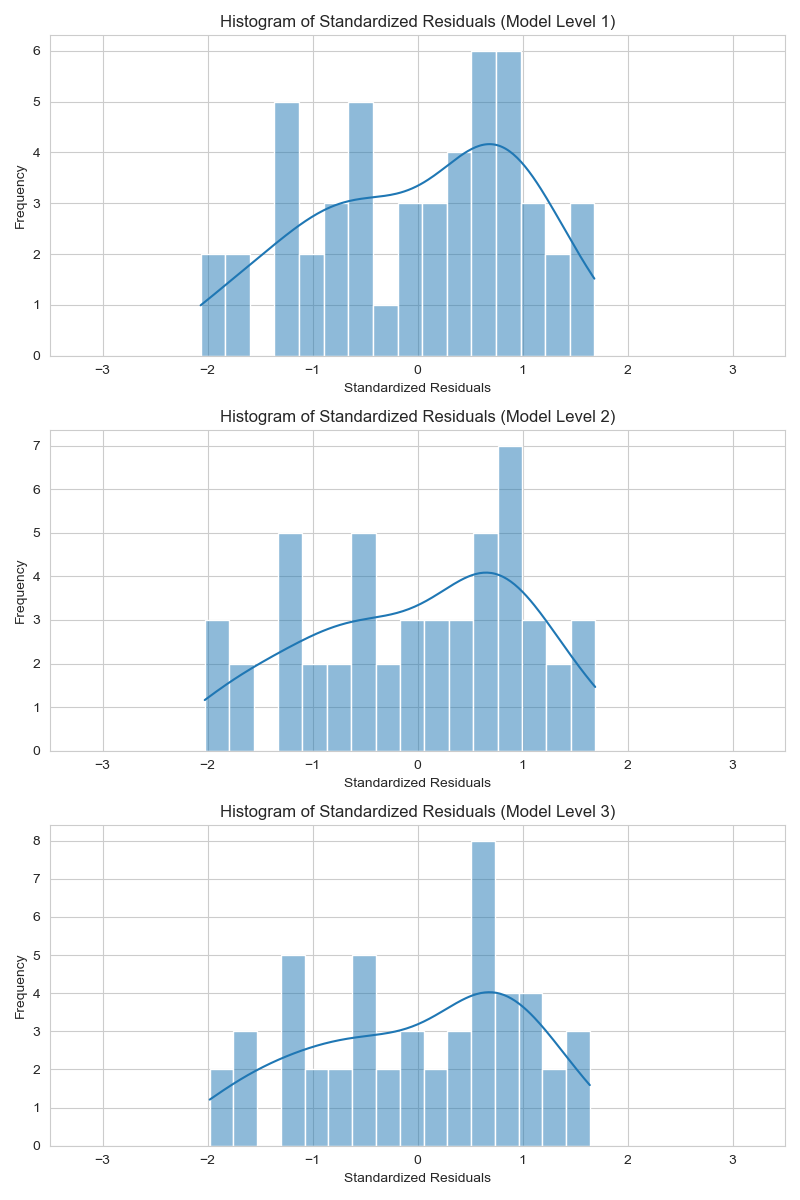
\includegraphics[width=\linewidth]{../plots/full_data/hierarchy8/histogram_std_residuals}
  \caption{Standardized Residuals Historgram}
\end{subfigure}%
\begin{subfigure}{.5\textwidth}
  \centering
  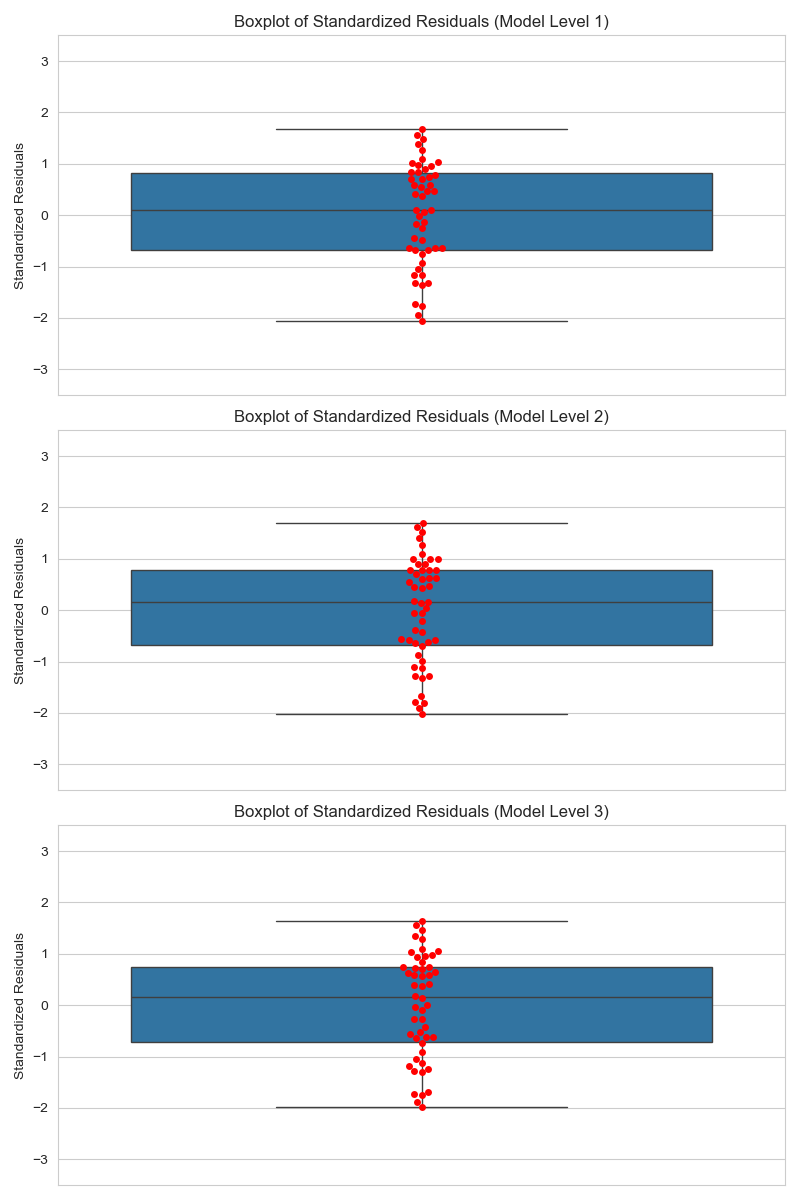
\includegraphics[width=\linewidth]{../plots/full_data/hierarchy8/std_residuals}
  \caption{Boxplot of Standardized Residuals}
\end{subfigure}
\end{figure}

\begin{figure}[H]
\centering
\begin{subfigure}{.5\textwidth}
  \centering
  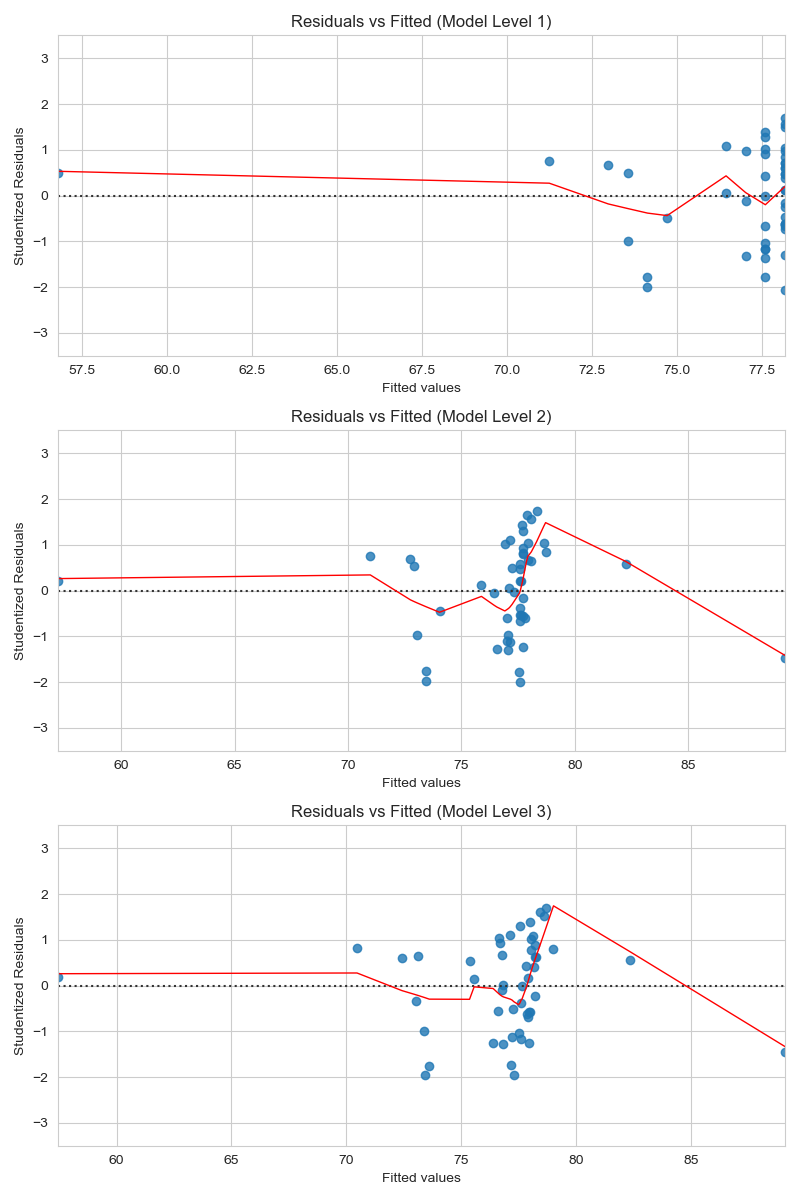
\includegraphics[width=\linewidth]{../plots/full_data/hierarchy8/studentized_residuals_vs_fitted}
  \caption{Standardized Residuals plot}
\end{subfigure}%
\begin{subfigure}{.5\textwidth}
  \centering  
  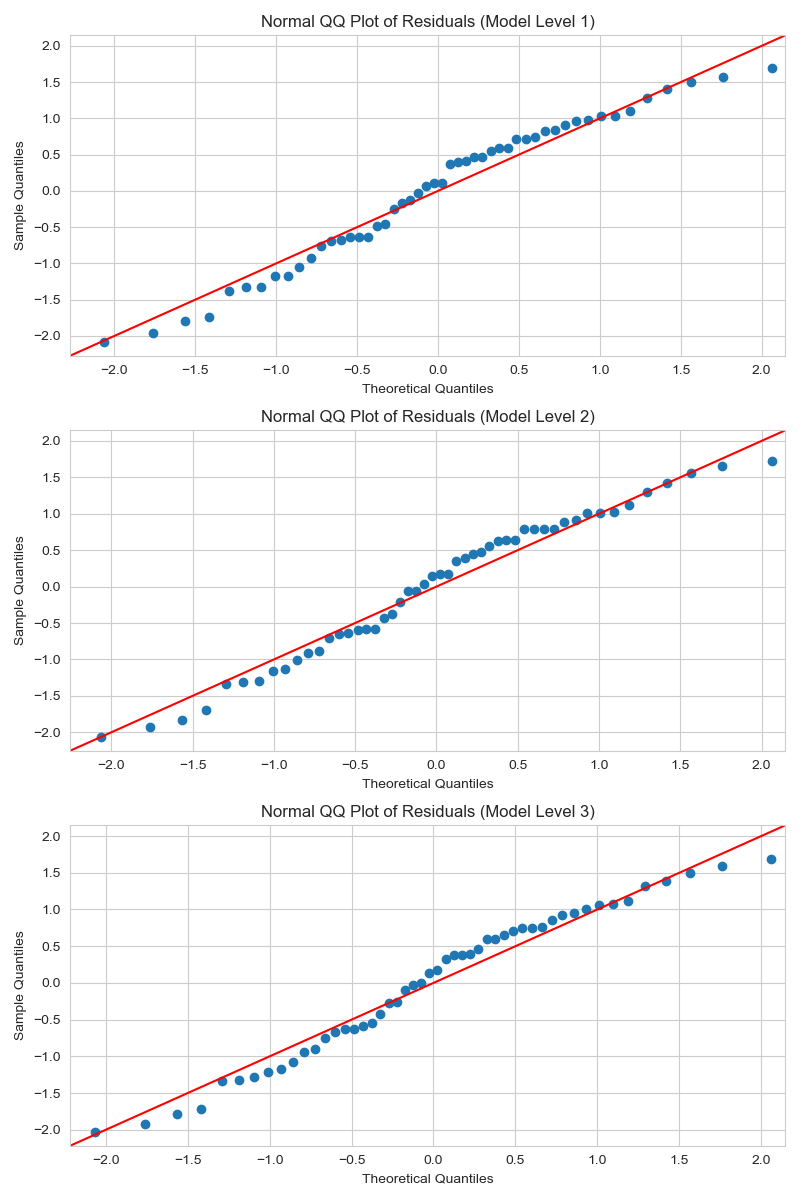
\includegraphics[width=\linewidth]{../plots/full_data/hierarchy8/qq_residuals}
  \caption{QQ plot of Standardized Residuals}
\end{subfigure}
\end{figure}

\begin{figure}[H]
    \begin{center}
    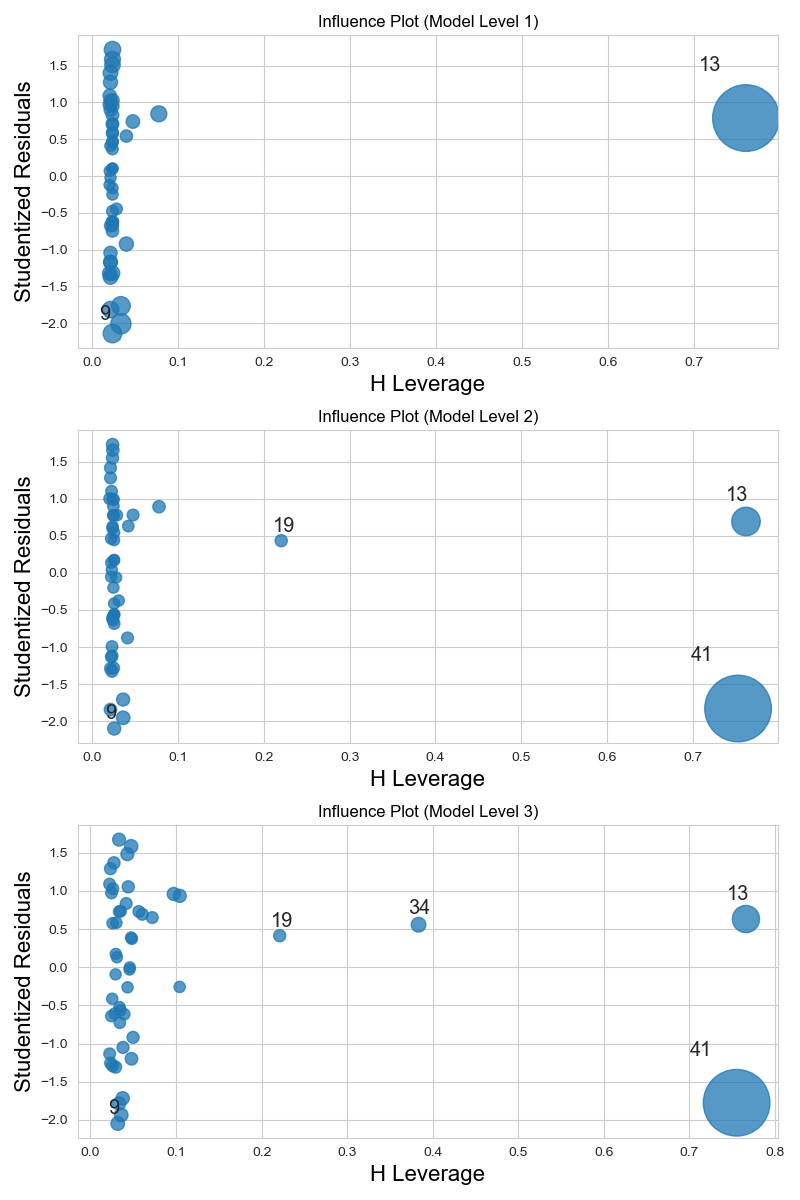
\includegraphics[width=0.5\linewidth]{../plots/full_data/hierarchy8/influence}
    \caption{Plot of influence of Different Points on the model}
    \end{center}
\end{figure}

\begin{figure}[H]
\centering
\begin{subfigure}{.5\textwidth}
  \centering
  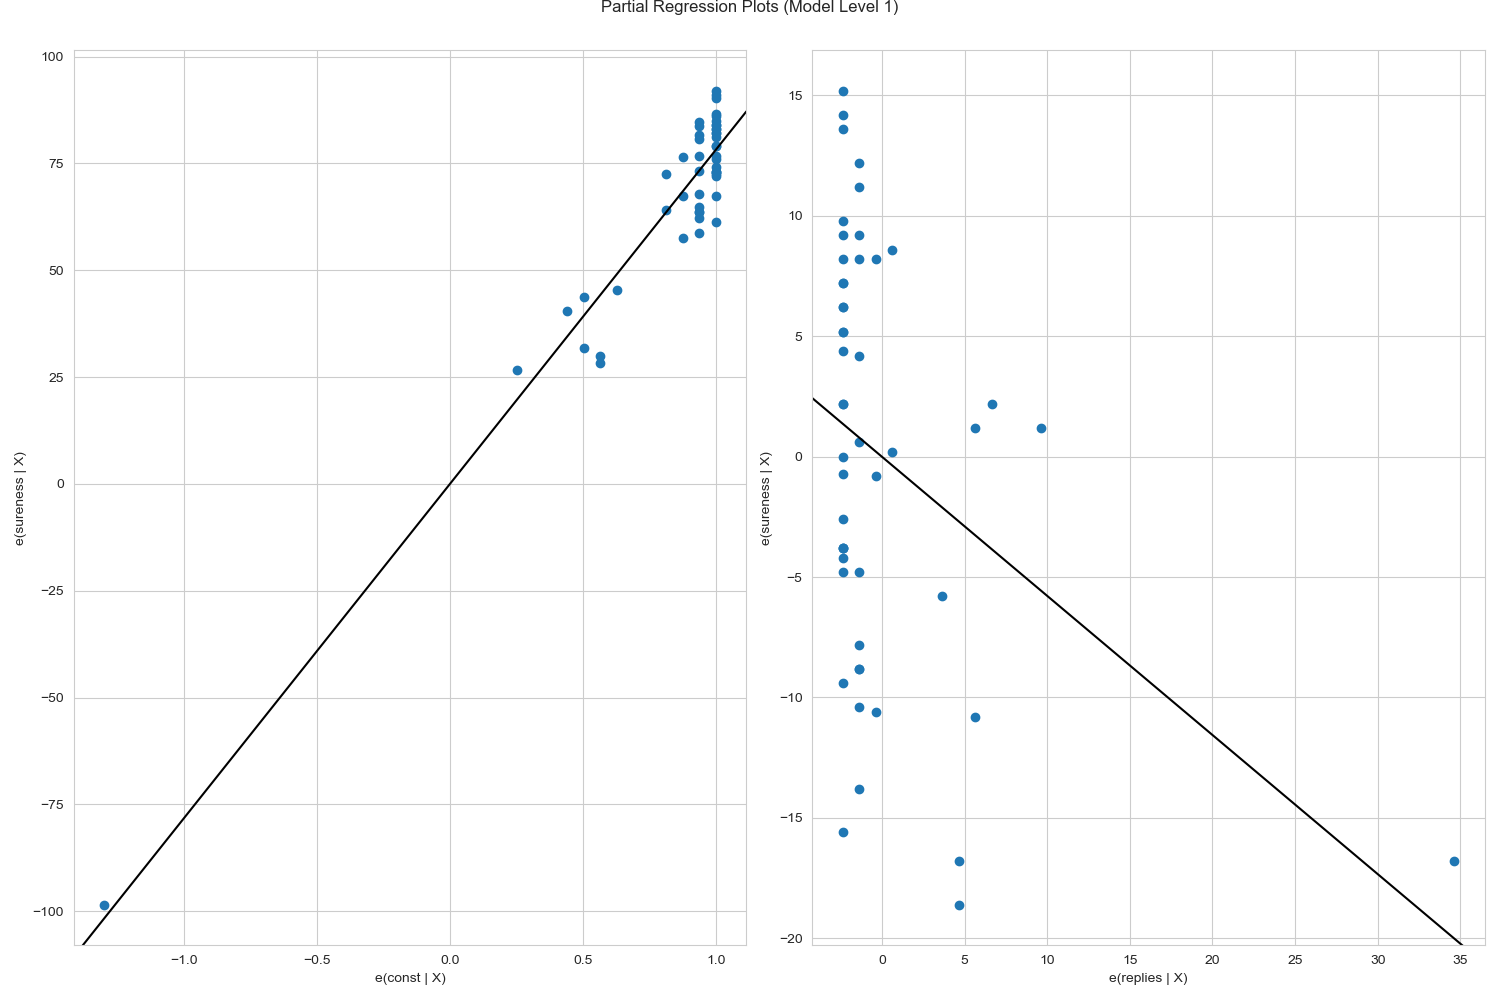
\includegraphics[width=\linewidth]{../plots/full_data/hierarchy8/partial_regression_0}
  \caption{replies}
\end{subfigure}%
\begin{subfigure}{.5\textwidth}
  \centering
  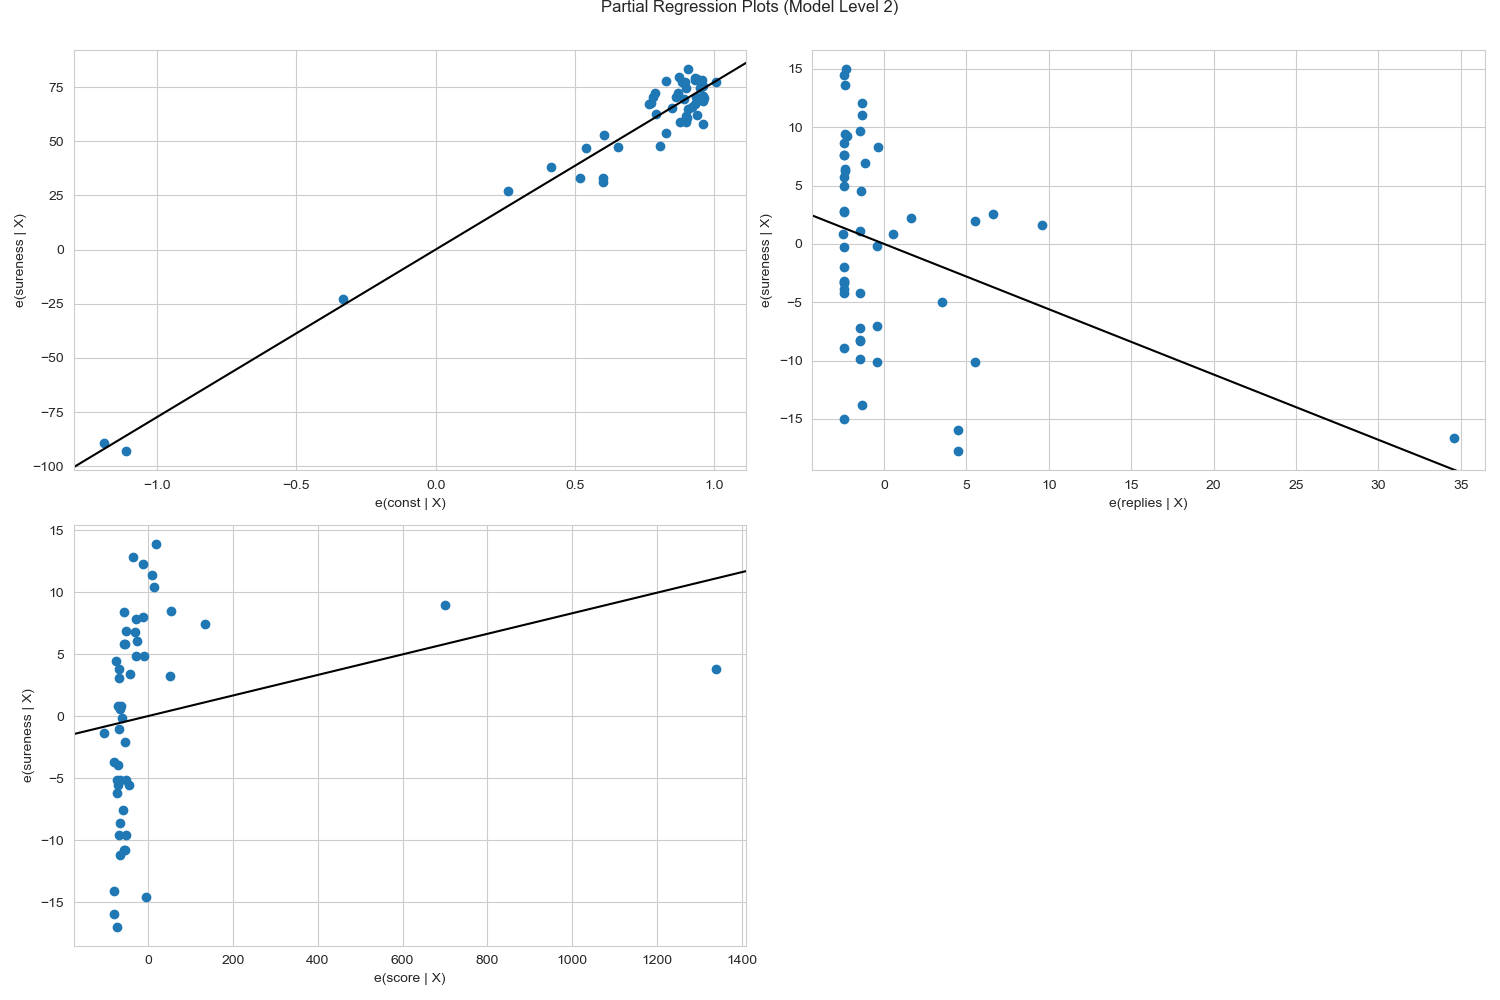
\includegraphics[width=\linewidth]{../plots/full_data/hierarchy8/partial_regression_1}
  \caption{replies; score}
\end{subfigure}
\begin{subfigure}{.5\textwidth}
  \centering
  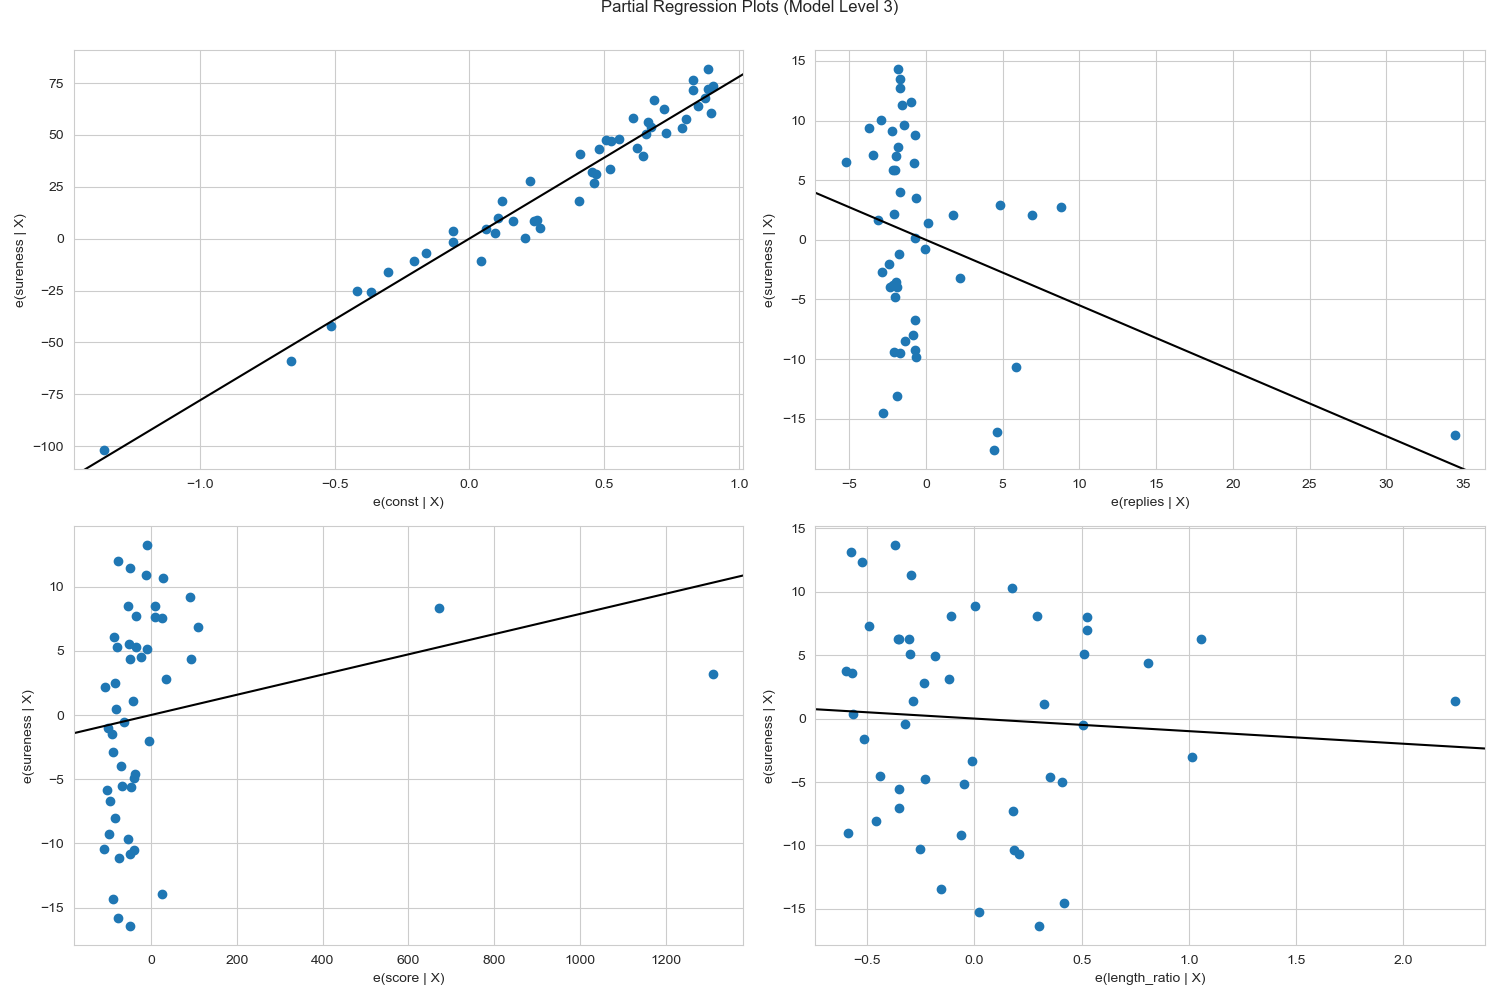
\includegraphics[width=\linewidth]{../plots/full_data/hierarchy8/partial_regression_2}
  \caption{replies; score; length ratio}
\end{subfigure}
\caption{Plots of Standardized Residuals as a function of each individual cue + constant}
\end{figure}

Plots of different cues and their effects on the final sureness:
\begin{figure}[H]
\centering
\begin{subfigure}{.5\textwidth}
  \centering
  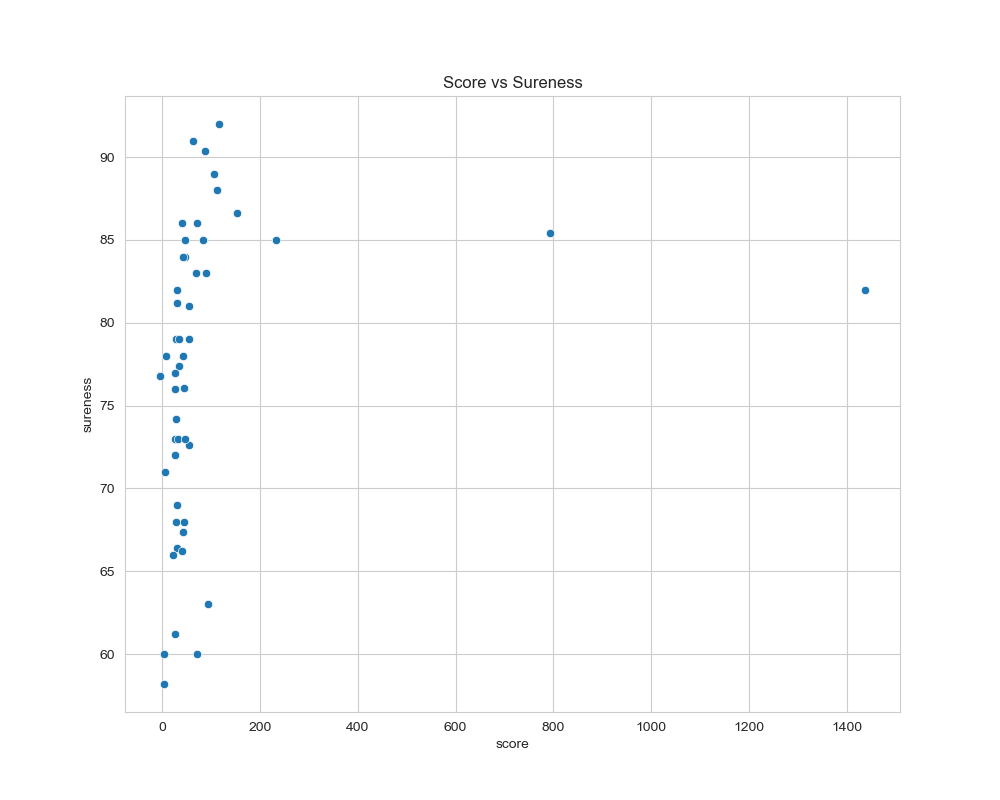
\includegraphics[width=\linewidth]{../plots/full_data/score_vs_sureness}
  \caption{Score - Sureness}
\end{subfigure}%
\begin{subfigure}{.5\textwidth}
  \centering
  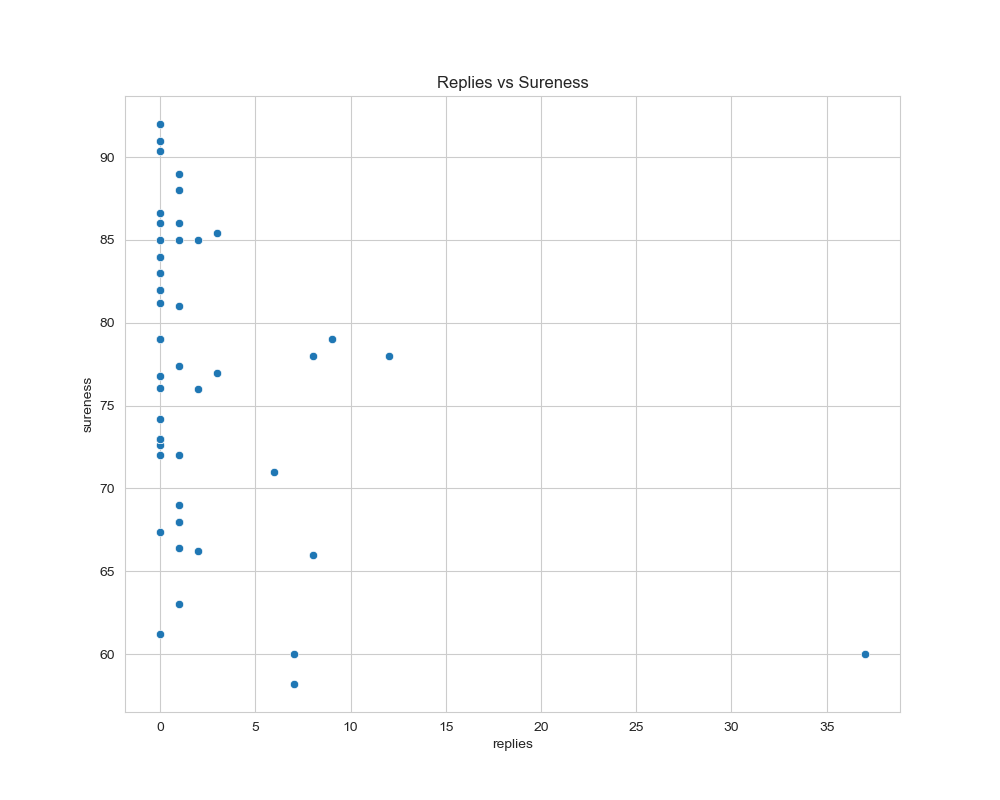
\includegraphics[width=\linewidth]{../plots/full_data/replies_vs_sureness}
  \caption{Replies - Sureness}
\end{subfigure}
\begin{subfigure}{.5\textwidth}
  \centering
  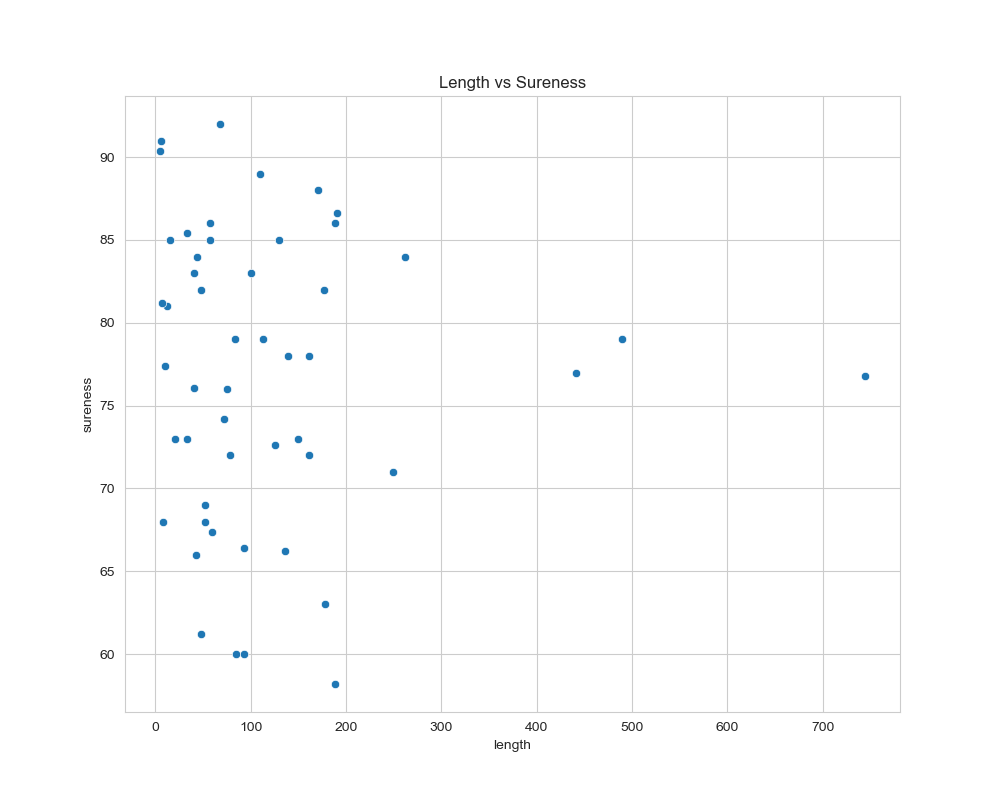
\includegraphics[width=\linewidth]{../plots/full_data/length_vs_sureness}
  \caption{Length - Sureness}
\end{subfigure}%
\begin{subfigure}{.5\textwidth}
  \centering
  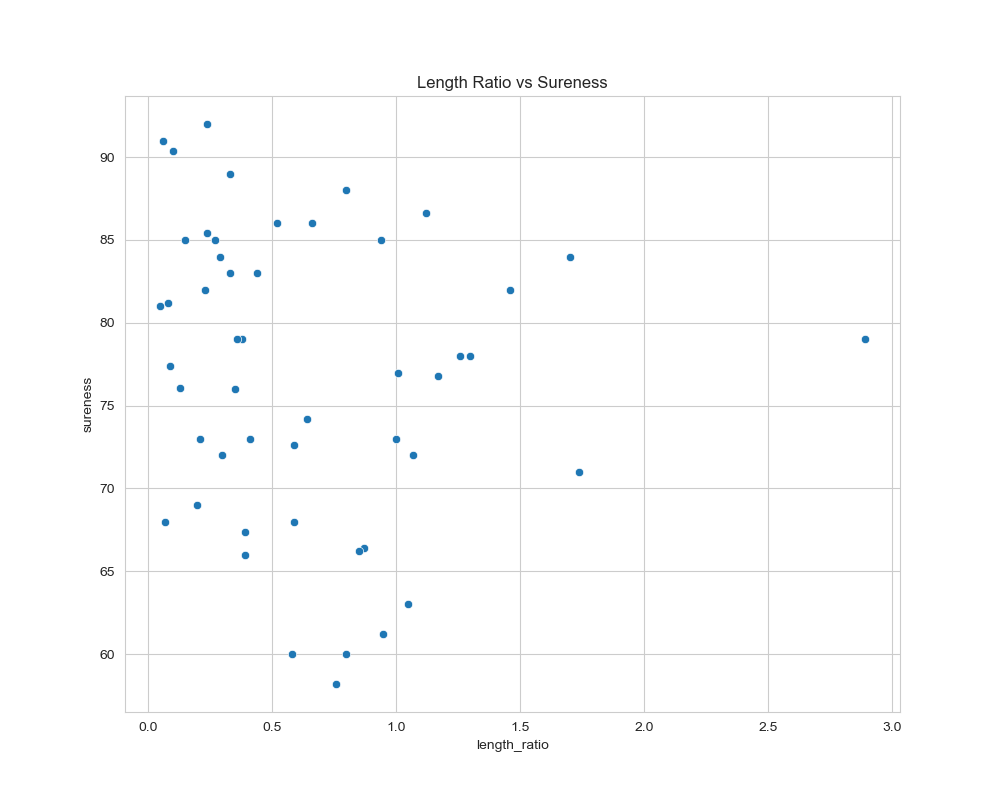
\includegraphics[width=\linewidth]{../plots/full_data/length_ratio_vs_sureness}
  \caption{Length Ratio - Sureness}
\end{subfigure}
\caption{Different Cues and their Effects on the final Sureness}
\end{figure}

\section{Conclusions}
We would like to preface all our conclusions by saying that we are happy to have encountered all of the problems that we did, both in the process of data collection (i.e. having to scrape a huge number of subreddits in order to get a required number of points) and in the process of data processing (i.e. models that do not learn well from the data, and linear regressions which are not valid to use.)\\
We believe that the process we underwent shows an authentic experience of trying to collect, label, and train on the data from the internet.
\subsection{Possible problems in data collection}
We have written at length about the problems which might arise from collecting data from internet forums in \hyperref[sec:inter_conclusions]{Intermediate Conclusions}, however we would like to linger on a few things.\\
\begin{itemize}
    \item Firstly, we have seen in all of the influence plots presented that there is at least one ourlier which strongly affects predictive power of the model. As we have not stored either the question or the answer texts, we cannot be sure why those points are outliers. Is it a comment/post by a troll or flamer, or is it a legitimate post with variance that we do not understand?
    \item Secondly, collecting data in a real world setting is very different from working with synthetic data produced in controlled experiments with precisely defined settings. Working with forums we involuntarily encounter a very complex dynamics of human communities, whose interactions are affected by time, current state of the world, and each other. It is unclear if it will be ever possible to clearly explain the data by the methods we have used here.
    \item And finally, we have collected both the data and labels in a very crude way: 
    \begin{itemize}
        \item Static rules of the form "has ?" or "contains 'help' " are not able to properly sort relevant questions from irrelevant ones. Moreover, we have not sorted the comments at all, which means that possibly there are comments with a high score/length/replies number, which have absolutely nothing to do with the question itself, and are only aiming at achieving community engagement.
        \item Additionally, when we have collected the comments, each question had a different "life-time". That is, some questions were new, and therefore the comments still had little engagement, while others were posted a few months previously. This too, may have greatly affected the results.
        \item Similarly to the previous point - there are differences between different forums. Some might have a much higher engagement than others; different tendency of people to like, reply or comment. Ideally there should be a way to normalize the results according to each of the responsible subreddits.
        \item Each label we have used for prediction was an average of opinions of 5 people, and it is unclear if it was enough to cancel the individual biases, or possibly could we have made them worse?\\
    \end{itemize}
    Ideally, such data collection pipeline should include an LLM step, which would selectively filter the questions and answers by their content. This might help to get a much cleaner data, but could also introduce a new source of bias.
\end{itemize}

\subsection{A few words on the BEVoCI results}
Fistly, we have clearly seen that for the \hyperref[sec:ffn_hlr]{explainability of the neural network}, the Hierarchical Regression approach hasn't worked at all. Even the best set of cues has an $R^2$ value of around 13\%, and if we look at the p-value of the test for validity of either the linear regression use, or addition of new cues, non of them surpasses the value of 0.05.\\
This is due, probably, to the fact that many of the assumptions which should hold to use linear regression in the first place are not true in this case - non of the cues holds the linearity assumption. Normality of residuals by Shapiro-Wilk test doesn't hold; and even the Rainbow test - which checks for linearity of a middle subsection of the points, holds with a relatively low p-value (null hypothesis is that there is linearity, therefore the higher - the better).

As to the analysis we have done on the full data - here too, we can see that the regression did not succeed. The best set of cues has an $R^2$ value of around 19\%, and out of all the cues only the 'replies' passes the linearity tests. 'replies' is also the only cue which passes the validity of use of linear regression test (with p-value of 0.0074); and addition of all others is not statistically valid.\\
It is interesting to note in this context that if we assume that replies is indeed a cue that is used by people to make their sureness prediction, it has a clear negative effect on the final label. We can put forward a hypothesis that the less coherent an answer (comment) is - the more pople would reply and express their disagreement. However, a similar hypothesis can be done in the other direction, therefore we are not sure how trustworthy these results are.\\
To stress this point even more, we could look again at the graph of sureness as a function of replies:
\begin{figure}[H]
    \begin{center}
    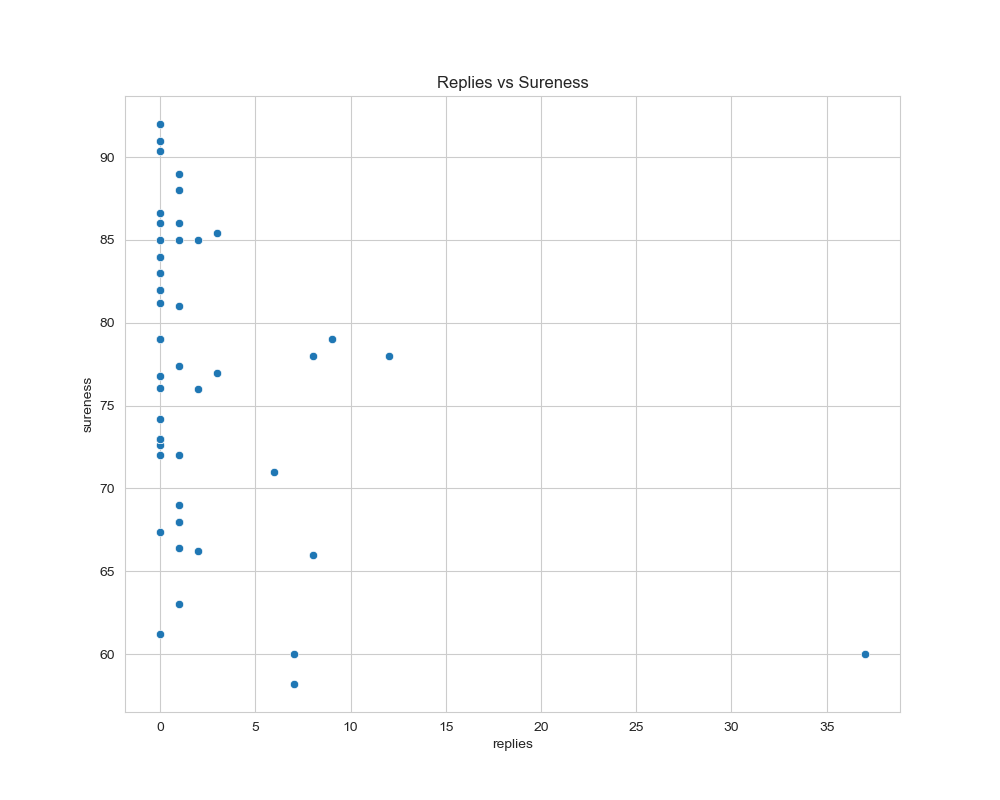
\includegraphics[width=0.6\linewidth]{../plots/full_data/replies_vs_sureness}
    \caption{Replies - Sureness}
    \end{center}
\end{figure}
It could be said that there is indeed a negative linear correlation between the replies cue and the sureness value. But in truth, there is a very high variance for any value of replies, and if we look at the histogram of the frequency of the replies:
\begin{figure}[H]
    \begin{center}
    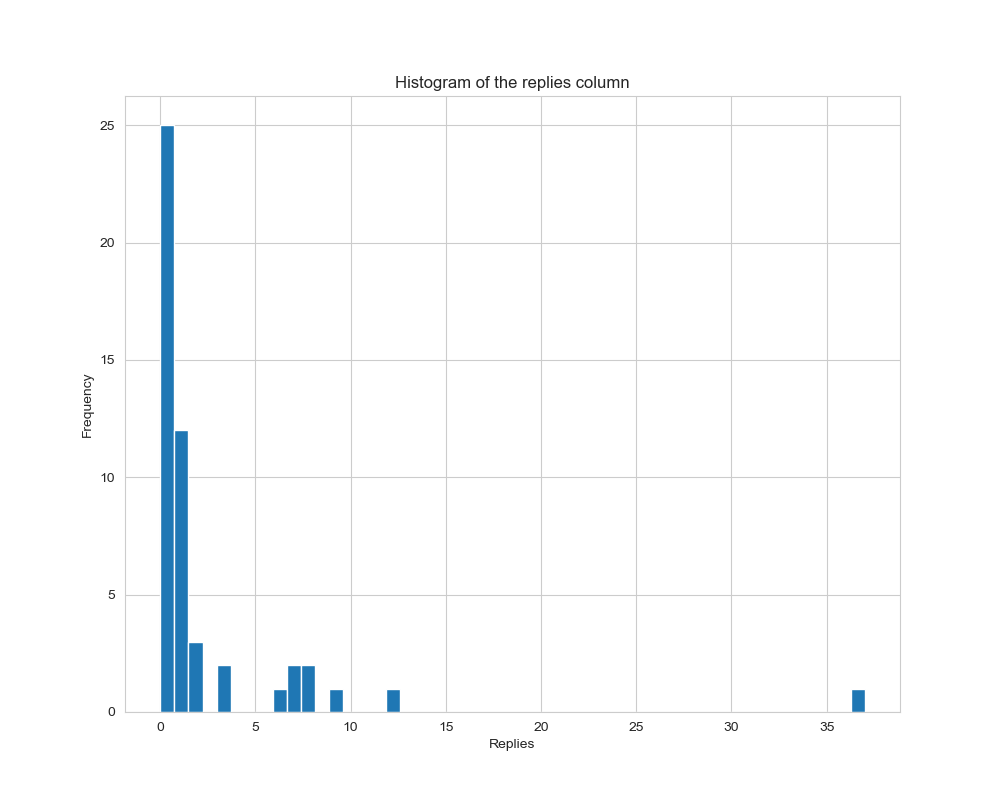
\includegraphics[width=0.6\linewidth]{../plots/replies_histogram}
    \caption{Replies - Sureness}
    \end{center}
\end{figure}
There are just many more points with lower reply values.\\

In order to say something for sure we would need many more points to explore.

\subsection{Final Remarks}
Doing this project is the first we have met the Hierarchical Linear Regression approaches, and we strongly believe that there is much promise to the BEVoCI methodology.\\ 
However, usefullness of the results produced by this method are limited to data with either true linear relations, or non-linear data with a low level of non-linear complexity.\\

Data collected from the internet exhibits many inherent correlations, and is in large a projection of complex social dynamics. It is yet to be seen whether some, or any, aspects of this dynamics could be usefully explained by the HLR methods.\\

Deep learning models, and specifically neural networks, are powerful, in large, due to the non-linear properties that they introduce through the different activation layers. We think that even if very simple networks could be explained by regression models (by the virtue of themselves being not far from linear), more complex networks would produce dynamics so non-linear that they would not be comprehensible with the help of BEVoCI. 

\end{document}  